\chapter{Complex Langevin dynamics of spherical dimers}
\label{chapter:langevin_dynamics}
\section{Overview}
Often in calculation of optical forces and scattering the
choice of target particle is often either a single sphere 
or a large agglomeration of spheres. In optical tweezing 
research the target particle is not guaranteed to be a 
sphere, instead either being an asymmetrical shape, or being 
a collection of smaller spheres.  

As an example, while working with dense colloidal suspensions, 
one often ends up trapping more than one sphere. Li and 
Arlt \cite{Li2008} studied the case of two microspheres 
trapped in a single OT and found that multiple trapped 
beads could be mistaken for a single trapped bead with an  
altered trap stiffness (see \ref{sec:harmonic_traps}). 
Theoretical studies on the case of two trapped microspheres 
by Xu~\textit{et~al.} \cite{Xu2005} employed a ray-optics 
based model to show that the two trapped beads are brought 
into physical contact with each other by optical forces 
and they also calculated the axial equilibrium positions 
of the two trapped beads as a function of their size. 
Experiments in \cite{Praveen2016} confirmed that the two 
trapped beads indeed experience different trap stiffnesses 
in the vicinity of the same potential well.
 
There are further discussions looking into the dynamics of 
a whole host of asymmetrically shaped particles (e.g. 
ellipsoids, cylinders, amorphous solids, disks, etc) 
\cite{Loudet2014, ShengHua2005, Chetana2022}, their results 
all showing that predicting the behaviour an arbitrary shaped 
particle comes with great difficulty due to the fact that the 
optical force is dependent on a greater number of variables 
such as orientation and size factors. While these have been 
noted as important factors, there has not been a concentrated
effort to discuss their impact over the course of a typical 
trajectory. 

With the initial goal of the project being to induce 
nucleation events via a rotating sphere, the aim of this 
chapter is to - in a limited capacity simulate and investigate 
the influence of a second particle being bound to our target 
sphere. The choice of a dimer, instead of an amorphous solid 
that might better represent a growing crystalline solid, 
allows us to consider how the dynamics of the aggregate change 
by varying a single parameter, namely the size ratio of the 
two spheres. Additionally, attempting to simulate an amorphous 
aggregate is rather difficult as calculating the optical force 
and torque is computationally slow. 
 
 In this chapter we will consider how the addition of a 
 second sphere changes the trapping dynamics by introducing 
 multiple equilibrium positions. In addition we demonstrate 
 that the angular dependency of the optical force allows for 
 multiple equilibrium orientations for a single particle. 
 Furthermore, we look at how dimers interact with circularly 
 polarised light, noting how our current understanding of 
 light and particle interactions does not accurately explain 
 the observed behaviour. We show that a dimer can undergo 
 gyroscopic precession by utilising this unique interaction 
 with circularly polarised light.  
 
%%%%%%%%%%%%%%%%%%%%%%%%%%%%%%%%%%%%%%%%%%%%%%%%%%%%%%%%%%%%%%%%%%%%%%%%%%%%%%
%%%%%%%%%%%%%%%%%%%%%%%%%%%%%%%%%%%%%%%%%%%%%%%%%%%%%%%%%%%%%%%%%%%%%%%%%%%%%%
\section{Simulation Details}
As a paradigmatic example, consider a dimer suspended in 
water ($n_p = 1.59, n_m = 1.33$) located at the focus of 
a Gaussian beam (more specifically a Laguerre-Gaussian 
beam of mode $[0,0]$, see \eqref{eq:incident}). The beam 
is focused by a objective with numerical aperture of 1.2.
The polarisation is defined using the Jones vector which 
describes the magnitude of the x and y components of the 
electric field (so the vector $[1.0, 0.0i]$ describes an 
electric field that only oscillates in the x direction). 
Unless stated otherwise the Jones vector is kept at $[1.0, 
0.0i]$. 

As a paradigmatic example, we study a simple spherical 
dimer composed of polystyrene, while there is the 
possibility of considering absorption we choose to keep 
the refractive index fixed at 1.59. The ratio of the two 
sphere radii is given by $a_{I}/a_{II}$ where $a_{I}$ is 
kept at $1\ \mu m$ unless specified otherwise. For 
simulations we assume that the dimer is suspended in water 
at room temperature ($T = 298K,\ \eta = 1.0x10^{-3}Pa\ s$).

In order to compute the magnitude of the Brownian forces we
need to know the dimer's diffusion tensor \textbf{D}. Unlike
for spheres where the translational and rotational diffusion 
coefficients are equal along all three Cartesian axis', a
dimer's translational and rotational diffusion is dependent
on whether we consider the its long or short axis. We use
the results from \cite{Nir1973} to compute the dimensionless 
diffusion tensor and then scale it according to the radius of
the largest sphere ($a_I$). The dimer's centre of diffusion
is located a distance of $a_I\zeta$ from the point of contact
between the two spheres, the coefficient $\zeta$ is based on
the size ratio of the two spheres. We use the centre of 
diffusion as the target origin that is provided to \textit{mstm}

Where $U_3$ represents the orientation vector that passes
through the centres of both sphere's (see \ref{sec:sim} 
for a full breakdown), $U_1$, and $U_2$ are orthogonal to 
$U_3$ but have no physical representation for a dimer. We 
can represent $U_3$ by it's spherical coordinates ($\theta$ 
and $\phi$), where $\theta$ is the angle between the 
orientation vector and the direction of propagation and 
$\phi$ as the angle between the orientation vector and 
the x-axis. We define the 'standard' orientation as 
being aligned with the direction of beam propagation 
direction ($\theta=0^\circ$) - and therefore the 'inverted' 
orientation is defined when the dimer is orientated against 
the direction of beam orientation ($\theta=180^\circ$) - see
fig~\ref{fig:paradigmatic} for a visual of the laboratory and
particle frame. 

Throughout this project we use the work of Vigilante \cite{Vigilante2020} 
to perform a systematic study of the dynamics demonstrated by 
asymmetric dimers in both plane and circularly polarised light. 
The simulations have two primary frames of reference that require 
explanation. Firstly, there is the laboratory frame which 
describes the coordinate system, we define the origin of our 
simulation as the focus of our trapping beam. While the choice in 
direction for the $x$ and $y$ axis are arbitrary the $z$ axis is 
specifically chosen so that it is aligned with the direction of 
beam propagation. 
\begin{figure}[h!]
	\centering
	\includegraphics[width=0.6\linewidth]{lab_frame.png}
	\caption{Ray scattering render of both the laboratory frame and 
		particle frame for a dimer and a Gaussian beam. The origin 
		of the laboratory frame is defined as the focus of the 
		trapping beam, with the positive $z$-axis being aligned with 
		the direction of beam propagation. The particle frame is 
		centred on the dimer's centre of mass with the primary axis 
		$U_z$ being aligned with the centres of the two spheres. Black 
		line is scaled to represent $1\ \mu m$.}
	\label{fig:lab_frame} 
\end{figure} 

Secondly there is the particle frame which describes the orientation 
state of the particle, orientations are reported as quaternions which 
can be readily transformed into rotation matrices. The dimer's 
orientation is given by a rotation matrix in the form: 
\begin{align}
	\begin{pmatrix}
		U_{1,x} & U_{2,x} & U_{3,x} \\
		U_{1,y} & U_{2,y} & U_{3,y} \\
		U_{1,z} & U_{2,z} & U_{3,z}
	\end{pmatrix}
\end{align}
The matrix describes the direction of the particles 3 orientation 
axis $U_1$, $U_2$, and $U_3$. The latter is oriented so that it 
is collinear with the centres of the two spheres; the direction 
of vector $U_3$ is such that it goes from the centre of $a_{II}$ 
to the centre of $a_{I}$. The origin of the 3 axis' is set on the 
particle's centre of mass, this is also used to define it's 
displacement from the origin of the laboratory frame. The diffusion 
tensor of the dimer is more complex than a sphere's as we must 
consider the rotational effects experienced by the dimer. We use 
the analytical solution of Nir \& Acrivos \cite{Nir1973}, where 
they provided the solution coefficients depending on the dimer's 
size ratio ($a_I/a_{II}$). Rather than recalculate the coefficients 
for every possible configuration of dimer we use a spline fitting 
function to approximate the diffusion tensor. 

We utilise a python library that utilises \textit{mstm} and
\textit{ott} to simulate the dynamical behaviour of spherical
aggregates. By specifying the optical properties of the target 
\textit{mstm} generates the targets T-matrix which can then be 
used by \textit{ott} to compute the optical forces generated by 
a focused beam. Using the Finite Differences approach we can solve
the Langevin Equation to take discrete time steps and update the 
dimer's position and orientation. A time step of $10 \mu s$ is 
used in line with previous works \cite{Vigilante2020}.

%%%%%%%%%%%%%%%%%%%%%%%%%%%%%%%%%%%%%%%%%%%%%%%%%%%%%%%%%%%%%%%%%%%%%%%%%%%%%%
%%%%%%%%%%%%%%%%%%%%%%%%%%%%%%%%%%%%%%%%%%%%%%%%%%%%%%%%%%%%%%%%%%%%%%%%%%%%%%
\section{Positional and Orientational dependence of Trapping forces}
\label{sec:eq_positions}
First, let us look at how the addition of a second sphere
changes how we go about looking for equilibrium positions
relative to the beam focus. Typically when trapping a target
particle we do not care where it is spacially in relation 
to the trap focus, we assume that it will end up in the same 
equilibrium position regardless. This assumption can not 
be taken when considering a dimer, or any aggregate of spheres.  

If we wanted to start from first principles and determine 
the trap strength on our target particle the first step 
would be to locate the equilibrium position relative to 
the trap focus. For a single sphere it is easy to enough 
to understand that its centre of mass will be drawn to 
focal point of the laser due to gradient forces, once there 
the force is analogous to a harmonic spring with a fixed 
trap stiffness (see fig.\ref{fig:harmonic_trap}). Now, if 
we consider instead a dimer, we now have two spheres both 
being drawn to the focus along by the same gradient force; 
in addition the scattering force is significantly more complex 
due to both spheres scattering the electromagnetic fields. 
This mutual scattering between individual spheres is what 
makes simulating spherical aggregates far more difficult 
compared to a single sphere, and even harder still to 
predict the position where the dimer's centre of mass is 
in equilibrium.

Because the scattering force is only significant in the 
direction of beam propagation \cite{Capitanio2002} we 
can assume there will only be a single potential well 
lying at the centre of the beam. Along the beam axis, 
such an assumption is no longer valid due to fact that 
spherical aggregates experience inter-particle scattering. 
This is a key reason for using \textit{mstm} as it 
accounts for that behaviour. The methodology for computing 
optical forces has been covered extensively for a number 
of different trapping conditions \cite{RanhaNeves2019}. 
So it is relatively easy to compute the trapping force 
and determine the equilibrium position by finding the 
position that minimises the net optical force and the 
local gradient is negative ($\delta F/\delta x < 0$) - 
we can assume that for a dielectric sphere the optical 
torque is negligible. For a dimer (or any arbitrary 
spherical aggregate), we now must consider both its 
position and orientation and find where the net optical 
force and torque are minimised. 

After computing its $T$-matrix via \textit{mstm} and 
supplying that to \textit{ott} we compute the optical 
force exerted by a $50\ mW$ laser via \eqref{eq:optical_force} 
in the axial direction while the dimer is in its 'standard' 
orientation. As expected we see a single point where 
the dimer will be in equilibrium, the linear fit in 
fig.~\ref{fig:paradigmatic}(a) indicates a that the 
force can be modelled as a harmonic potential close to 
the equilibrium position ($F_z\approx-\kappa_z z$). 
The second point where the axial force goes to 0 cannot 
be considered as equilibrium position as the positive 
gradient indicates that the trap is unstable unless 
Brownian motion is ignored. 

We repeated the same calculation but now while the 
dimer is in its 'inverted' orientation, instead of 
a single point where the optical force is minimised 
we see that there are instead two separate equilibrium 
positions, one above the focus and one below the 
focus. In this particular example the two positions 
are far enough apart that both can be considered as 
separate harmonic traps.    
\begin{figure}[h!]
	\centering
	\begin{subfigure}{.65\linewidth}
		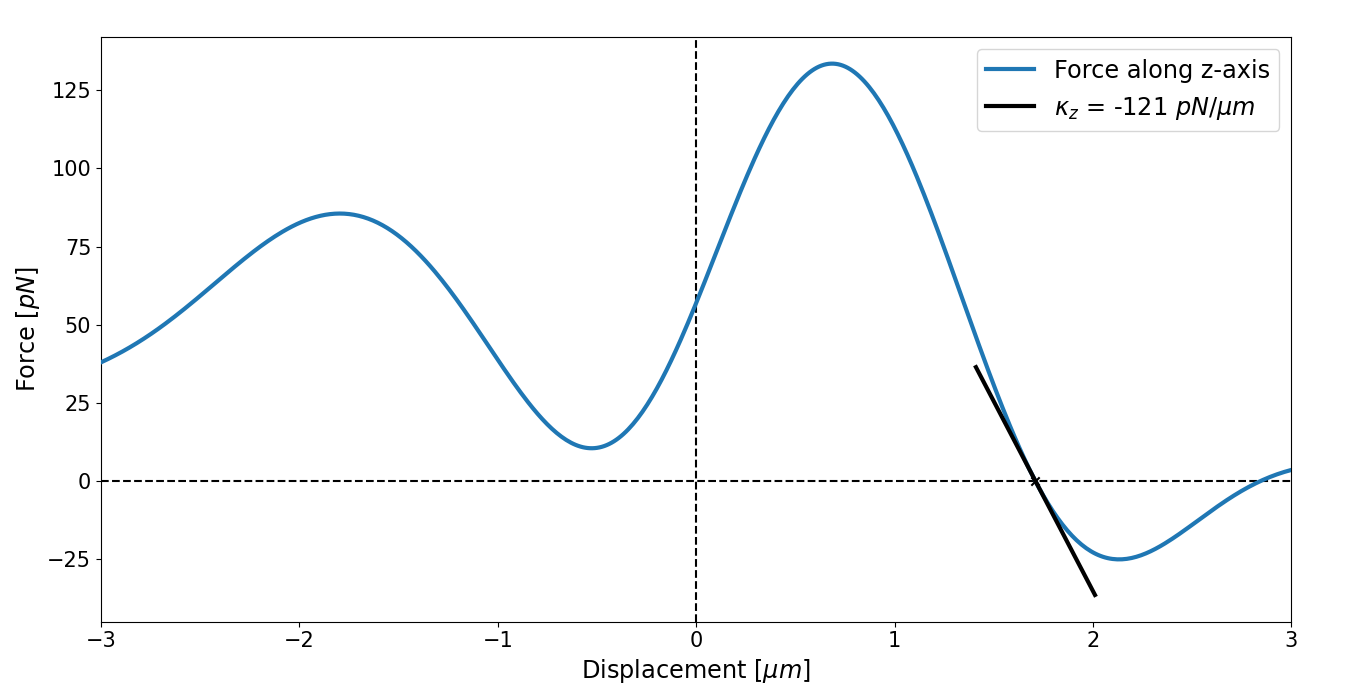
\includegraphics[width=\linewidth]{lam=2_theta=0.png}
		\caption{}
		\label{lam=2}
	\end{subfigure}\hfill % <-- "\hfill"
	\begin{subfigure}{.25\linewidth}
		\centering
		\raisebox{60pt}[0pt][0pt]{\makebox{}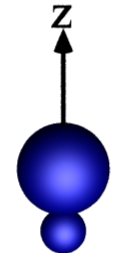
\includegraphics[width=0.3\linewidth, keepaspectratio]{theta=0.png}}
		\label{large over small}
	\end{subfigure}
	\medskip
	\begin{subfigure}{.65\linewidth}
		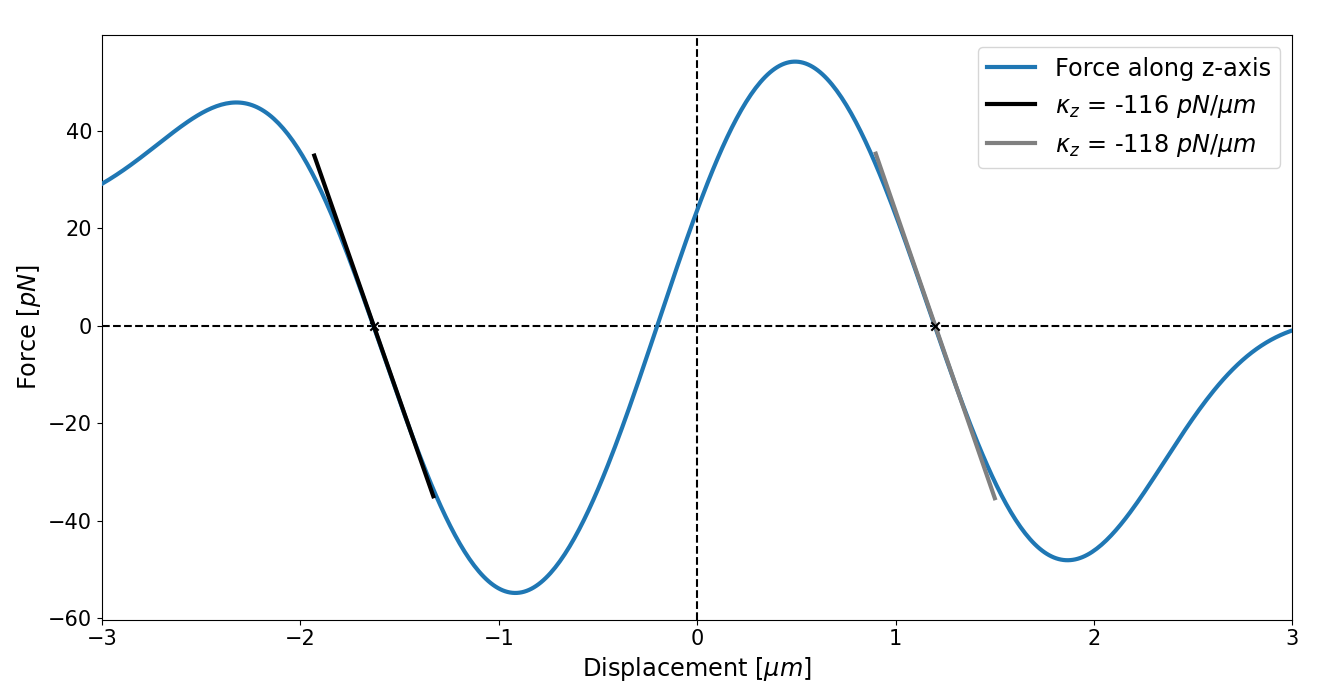
\includegraphics[width=\linewidth]{lam=2_theta=180.png}
		\caption{}
		\label{lam=2_inverted}
	\end{subfigure}\hfill % <-- "\hfill"
	\begin{subfigure}{.25\linewidth}
		\centering
		\raisebox{40pt}[0pt][0pt]{\makebox{}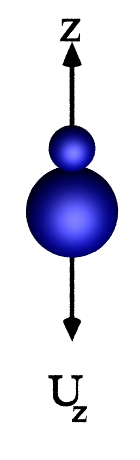
\includegraphics[width=0.3\linewidth, keepaspectratio]{theta=180.png}}
		\label{small_over_large}
	\end{subfigure}
	\caption{Plots of force vs displacement of the 
		centre of mass of the dimer (µm) for the 
		case of a dimer of size ratio 2. (a) is the 
		case where the dimer is in its' 'standard' 
		orientation, where the dimer is trapped at 
		$z = 1.71\ \mu m$. (b) is the case where the 
		dimer is in its' 'inverted' orientation, the 
		dimer is trapped at two positions: $z = 1.20\ 
		\mu m$ \& $z=-1.63\ \mu m$. On the left are 
		renders to visualise the dimer orientation 
		are shown below each plot. The black lines 
		on each force-curve is a linear fit with the 
		slope being reported as the trap stiffness in 
		the legend.}
	\label{fig:paradigmatic}
\end{figure}

This is different to a single sphere, namely in that a
single sphere should only have one equilibrium position
and that it is much closer to the trap focus ($\approx
0.05\mu\ m$ from the focus). This is also not similar 
to other works where random clusters of spheres have 
been shown to oscillate between stable points 
\cite{Vigilante2020}.

We can see that both equilibrium positions have 
comparable axial trap stiffness ($\kappa_z$), 
however the difference in the transverse trap 
stiffness ($\kappa_x$) is far more noticeable. 
The same dimer was trapped at each of the axial 
equilibrium positions and the transverse force was 
evaluated. While in all three cases the dimer can be 
trapped the linear range where that would typically 
associated with a stable trap is far narrower in the 
'standard' orientation compared to the 'inverted' cases. 
This highlights one of the challenges involved with 
studying asymmetric particles, even though its a 
simple enough process to trap them they maybe 
characterised very differently depending on their 
relative position and orientation towards the focus. 
This can have a significant impact on rheological 
studies - or attempting to probe any local property 
- as the variance in trap strength can result in 
large errors over repeated measurements. 
\begin{figure}[h!]
	\centering
	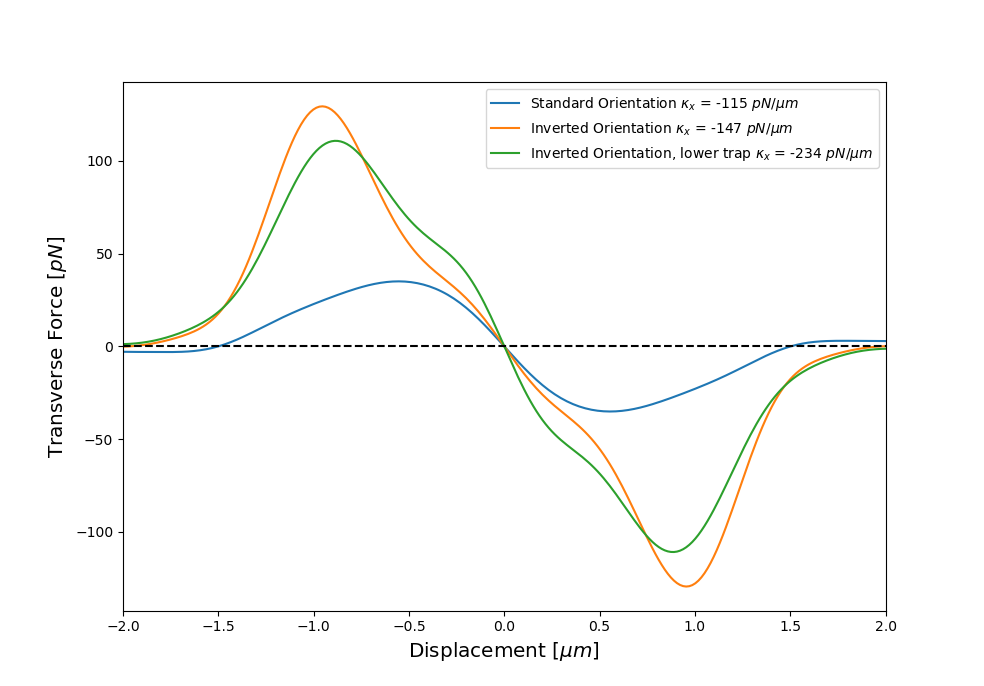
\includegraphics[width=\linewidth]{transverse_force.png}
	\caption{Plots of force vs displacement of the dimer's 
		centre of mass spheres, where a positive force 
		indicates the dimer is directed right on the x-axis, 
		and vice versa for a negative force. The same simulation 
		parameters are used here as in fig~\ref{fig:paradigmatic}
		(a) and (c). The blue curve representing the force 
		response for a dimer in its standard orientation, orange 
		being the inverted case, and green the same case but 
		placed below the focus.}
	\label{fig:transverse_force}
\end{figure}

\newpage
For completeness the harmonic traps were located for dimers
across a range of size ratios - from $a_{I}/a_{II} = 1$ to 
$a_{I}/a_{II}=10$ - while also recording the trap stiffness 
for each trap. The same simulation parameters are used here 
as for figures \ref{fig:paradigmatic} \& \ref{fig:transverse_force}. 
As shown in Fig.~\ref{fig:eq_positions} $a_{II}$ decrease 
the dimer begins to approximate a single homogenous sphere 
- at least in terms of location and trap strength. However, 
for intermediate sized dimers (between $a_{I}/a_{II} = 1.1$ 
to $a_{I}/a_{II}=4$), a second equilibrium position is found 
below the trapping focus. We should note that there are also
unstable traps that exist, these are also depicted in 
fig.~\ref{fig:eq_positions}. While the optical force
is zero at these positions the gradient $\delta F_z/\delta z$
is positive and so any Brownian motion would displace the 
dimer, either ejecting it from the optical trap or letting
it be drawn towards another harmonic trap. 
\begin{figure}[h!]
	\centering
	\begin{subfigure}{0.85\linewidth}
		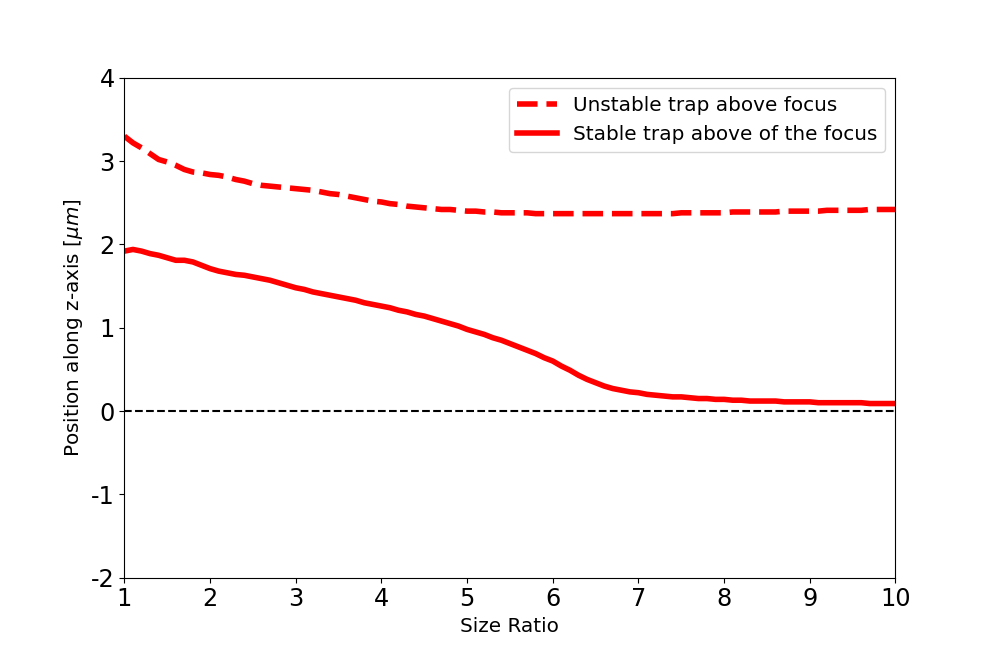
\includegraphics[width=\linewidth]{Equillibrium_positions.png}
		\caption{}
		\label{eq_pos}
	\end{subfigure}\hfill % <-- "\hfill"
	\medskip
	\begin{subfigure}{0.85\linewidth}
		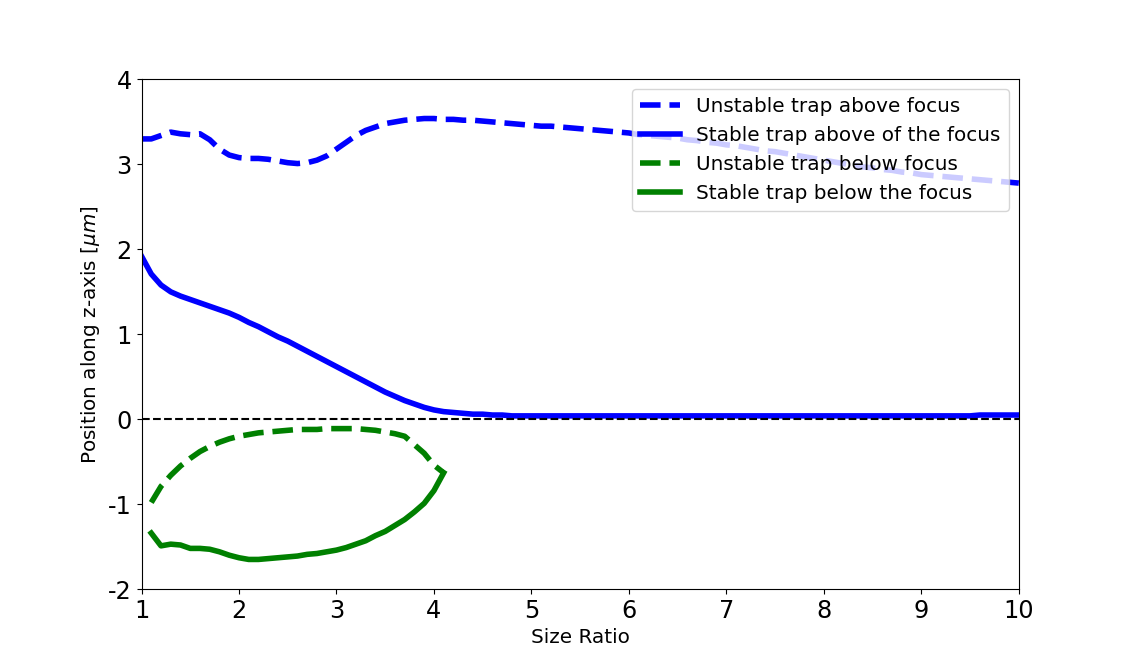
\includegraphics[width=\linewidth]{Equillibrium_positions_inverted.png}
		\caption{}
		\label{eq_pos_inverted}
	\end{subfigure}
	\caption{Equilibrium positions of optically trapped dimers 
		with varying size ratio, dashed lines represent unstable 
		traps whereas solid lines are for stable equilibrium 
		positions. (a) shows that dimers while in their 
		'standard' orientation will always have a single 
		equilibrium position. (b) shows that when the same dimer 
		is in its' 'inverted' orientation can be trapped in two 
		axial positions, one below the focus and one above the 
		focus.}
	\label{fig:eq_positions}
\end{figure}

Previous work using the ray-optics model have confirmed even 
in the case that two spheres begin separated the electric field 
will align the particles as such that they make contact and 
are trapped together about a single trapping position 
\cite{Xu2005}. Furthermore it has been shown through proper 
manipulation of the Gaussian or Bessel beam modes that any 
number of trapping potentials can be developed 
\cite{Shahabadi2020} for nanoparticles. This result however, 
is the first example of an orientation dependent trapping 
situation using only a $TEM_00$ beam. Typical experimental 
arrangements cannot determine much information on the axial 
position of a trapped particle relative to the trap focus; 
this result indicates not only that dimers can be trapped 
in multiple axial positions but also their trapping behaviour 
is heavily dependent on the axial position. As such it is 
necessary that positional information in the z-axis can be 
elucidated if multiple spheres are trapped simultaneously. 

\newpage
\section{Non-trivial basins of attraction}
\label{sec:off-axis}
As mentioned previously in \ref{sec:opt_torque} the 
torque applied to an anisotropic scatterer can be 
broken down into two categories: torque generated 
from the field polarisation and torque generated 
by the gradient force of the electric field. The 
former is generally only applicable for objects 
that are birefringent whereas the latter is 
applicable to dimers due to their elongated shape.
Since both spheres are attracted towards the centre
of intensity via the gradient force a dimer will 
experience a restoring torque that keeps the it
in an equilibrium orientation. For any elongated 
particle the torque is minimised when the long 
axis is aligned either parallel or perpendicular
with the direction of the electric field. In this 
section we try to find equilibrium configurations 
(positions and orientations where both the optical
force and torque are minimised).

Computing the equilibrium positions when a dimer is 
aligned with the electric field is relatively simple 
as the orientational torque is minimised (see Eq.
\ref{eq:opt_torque}). Meaning once trapped the 
dimer is unlikely to change orientation enough to 
escape the trap. Regardless, that does not rule out 
the possibility that there is a stable configuration 
where the orientation not strictly vertical, in fact 
most experimental work with symmetric nano-dimers will 
trap them lying perpendicular to the beam direction 
\cite{Ahn2018, Reimann2018}. Unlike in Sec.~
\ref{sec:eq_positions} we cannot simply compute the 
optical force and torque as the parameter space is too 
large and determining if a particular position and 
orientation is stable is not clear based solely on 
force and torque measurements \cite{Bui2017}. Using 
the same simulation parameters as before we ran a 
number short simulations (total simulation time was 
$0.005$ s) with the laser power increased to $500\ mW$. 
Each simulation started with the dimer in a different 
starting position and orientation, due to the high 
laser power the dimers either escaped the trap or 
were stably trapped. We chose to only consider the $z-
\theta$ phase space in order to simplify the explanation,
considering all possible parameters would increase the 
simulation time significantly. The $z-\theta$ phase space 
can be divided into different regions depending on which 
equilibrium configuration is reached.
\begin{figure}[h!]
	\centering
	\begin{subfigure}{0.67\linewidth}
		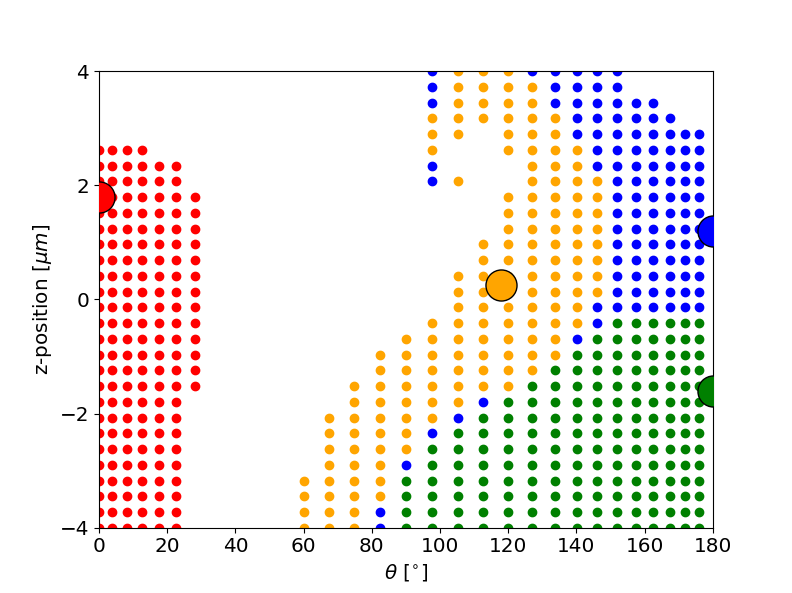
\includegraphics[width=\linewidth]{off_axis_trap.png}
	\end{subfigure}
	\begin{subfigure}{0.32\linewidth}
		\raisebox{0pt}[0pt][-10pt]{\makebox{}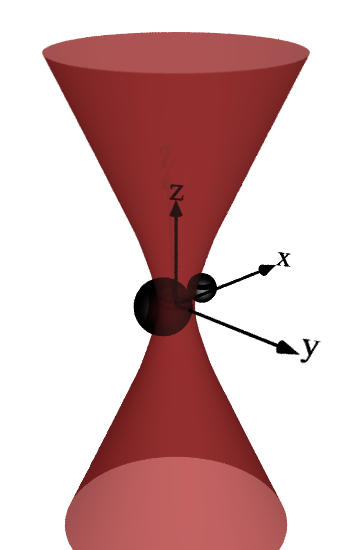
\includegraphics[width=\linewidth, keepaspectratio]{off_axis_render.png}}
	\end{subfigure}
	%\captionsetup{hangindent=2.35cm}
	\caption{Map of $z-\theta$ phase space using a dimer 
		of size ratio 2 with a laser power of 500 mW 
		($\theta=0^\circ$ is the 'standard' orientation 
		and $\theta=180^\circ$ is the 'inverted' 
		orientation). The stable configurations are 
		indicated by the larger circles and the 
		starting conditions are colour coded to match 
		the stable point they end up in. Right hand 
		render shows a dimer in its off-axis configuration.}
	\label{fig:off_axis}
\end{figure}

Where the each starting location is colour coded to
match the final equilibrium position reached, empty
regions indicate that the trap was escaped. As 
expected we see that the dimer has three separate 
traps when the dimer is close to its vertical 
orientation, similar to what we see from figs.~
\ref{fig:paradigmatic} and \ref{fig:eq_positions}. 
When the beginning orientation is close to horizontal 
there exists a $4^th$ harmonic trap. Each of these 
traps, has its own 'basin' of attraction around 
which the dimer is drawn into, the strange shape 
of these basins is likely due to how the asymmetric 
shape interacts with the optical trap.

Interestingly while the trap strength of these off-axis 
configurations are similar in magnitude to the vertically 
aligned dimers, but when the laser power is lowered 
(around $5\ mW$) the traps appear metastable. With the 
vertical configurations even after $30\ s$ of simulation
time the dimer is still trapped whereas the off-axis 
configuration can be escaped after only a few seconds of
simulation time. The suggested that the configuration is 
metastable is due to the increased rotational freedom. 
Similar configurations have been explored with ellipsoids; 
Zhu \textit{et al.} looked at the dynamics of various 
elliptical particles and found that regardless of shape or 
initial orientation the particle would tend towards either 
a purely vertical or purely horizontal orientation 
\cite{Zhu2021}. However, in our case the dimer never returns
to a vertical orientation, suggesting their is a potential 
barrier separating the different configurations. In order
to build a better understanding of the potential landscape 
we need to consider how the force and torque vary for a 
dimer in the $z-\theta$ phase space.  

\subsection{Force-Torque landscape of an arbitrary dimer}
We use \textit{ott} to compute the optical force 
and torque for the same dimer as used in fig.~
\ref{fig:off_axis} in different positions or 
orientations, this is depicted in fig.\ref{fig:force_torque}. 

The optical torques reported by \textit{ott} are
about their respective axis - so $T_x$ is the torque
that rotates the dimer about the x-axis in the particle
frame. 

The magnitude of the force and torque are indicated
by the colour intensity, with white indicating either
zero force or torque. This helps show where a
dimer may end up in equilibrium by finding 
where both the torque and force go to 0.
\begin{figure}[h!]
	\centering
	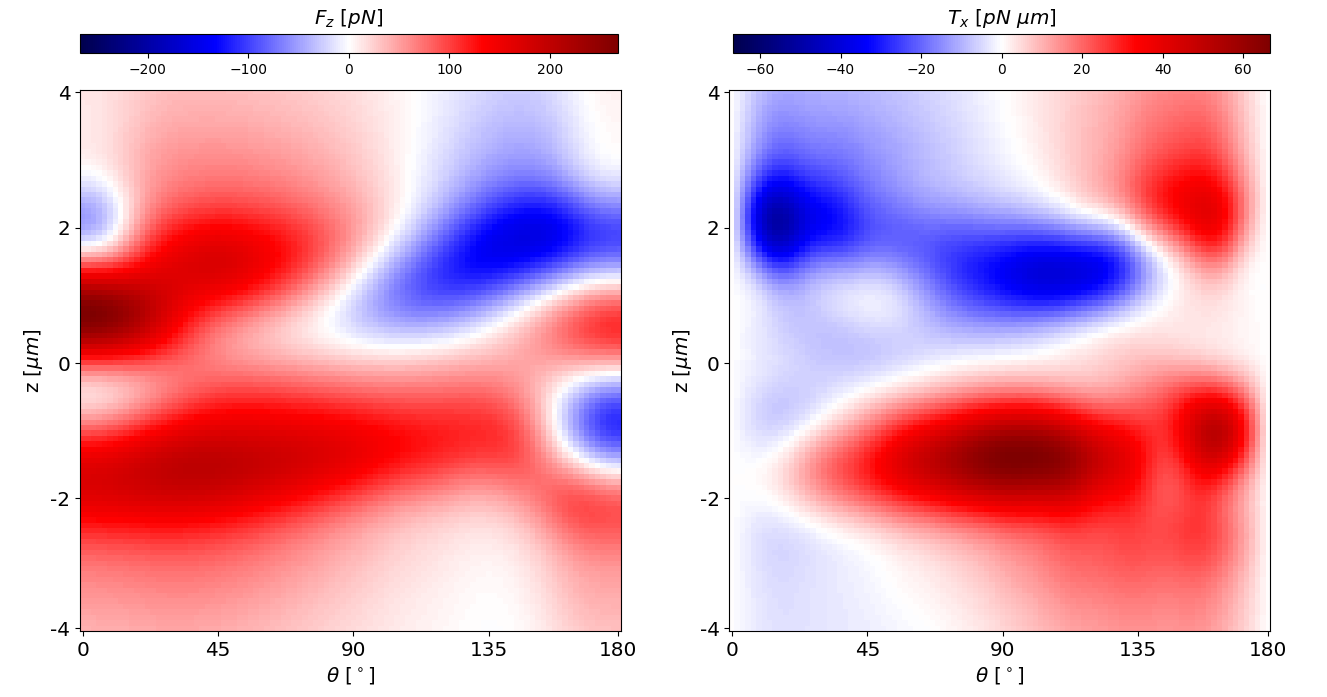
\includegraphics[width=\linewidth]{force_torque.png}
	\caption{Force-Torque landscape over the $z-\theta$ 
		phase space with a dimer is a size ratio of 2, 
		laser power of 100mW. Left: 2D plot of the 
		optical force in the axial direction as a 
		function of position and orientation. Right: 
		2D plot of the optical torque about the x-axis 
		as a function of position and orientation.}
	\label{fig:force_torque}
\end{figure}

The force and torque landscape provides some insight 
into how the dimer can inhabit an off axis equilibrium
orientation. Firstly, lets consider a typical trap, 
while the dimer is close to vertical; in all of these 
cases the optical force and torque directs the dimer 
back to the configuration. In this case the potential 
well is positive whether the dimer moves along the 
z-axis or is rotated. We can assume that in both cases
the translational and rotational stiffnesses are close
enough to be modelled as harmonic potentials.

However when in an off-axis configuration ($z\approx0$ 
\& $90^\circ\le\theta\le115^\circ$) the optical torque 
is working against the optical force, trying to move it 
out of equilibrium while the optical force returns it to 
equilibrium. This means that the potential well is more 
akin to a saddle point, the only reason that the optical
trap is not escaped immediately is because the the 
translational trap stiffness is significantly greater than
the gradient of the optical torque ($\kappa_z\gg\kappa_
\theta$). Therefore it is more accurate to say that the 
trap is not metastable, as when the trap is escaped it 
is not because the Brownian displacement is greater than
the potential well, rather the dimer is randomly 
traversing along the x-axis (aka random Brownian 
rotation) and has escaped the translational potential 
well. 

The force-torque landscape also provides an explanation
to the boundaries between the different trapping 'basins'
in fig.~\ref{fig:off_axis}. The first point of interest 
is the 'dead zone' around the orange basin. Looking at 
fig.~\ref{fig:force_torque} we can see that around that
region ($z \approx 2.5\mu$ \& $\theta\approx 110^\circ$)
the optical torque changes sign as you move closer to 
the trap focus. There is no clear physical reason why
the optical torque change direction so abruptly but a 
consequence of it is that dimers that are too close to 
this region of the torque landscape are ejected from 
the optical trap as the are drawn down towards the trap
focus.

The only pellicular result is the observation that the 
blue basin can still be reached well below the trap 
focus. As shown by fig.~\ref{fig:off_axis} there are a 
handful of starting configurations that end up in the 
upper trap while in the inverted orientation. Even 
consulting fig.~\ref{fig:force_torque} does not indicate
any reason why this occurs. The only conclusion we can 
draw is that the orange and green basins of attraction 
are small enough that it is possible for a dimer to 
avoid both. 
%%%%%%%%%%%%%%%%%%%%%%%%%%%%%%%%%%%%%%%%%%%%%%%%%%%%%%%%%%%%%%%%%%%%%%%%%%%%%%
%%%%%%%%%%%%%%%%%%%%%%%%%%%%%%%%%%%%%%%%%%%%%%%%%%%%%%%%%%%%%%%%%%%%%%%%%%%%%%
\section{Continuous rotational motion in circularly polarised light}
One aspect that has yet to be covered in depth with regards 
to spherical aggregates of any construction is their interaction 
with circularly polarised light. For homogenous spheres the 
optical torque is regarded as being negligible as the spin 
density cannot impart angular momentum while propagating in a 
homogenous medium. Dimers however, have been shown to experience 
an optical torque \cite{Vigilante2020, Ahn2018, Reimann2018} 
while trapped in a circular polarised beam. In our simulations 
we found that dimers would rotate about their long axis when 
trapped in circularly polarised light. In this section we want 
to discuss how this behaviour is influenced by size, position, 
and orientation; and furthermore, we wish to address possible 
explanations for this behaviour, as none of the current
theories into optically induced rotation seem plausible.

\subsection{Polarisation Dependency on Dimer trajectory}
\label{sec:rot_pol}
In their paper Vigilante \textit{et al} attribute the 
rotational motion to the anisotropic shape of the dimer
\cite{Vigilante2020}. Anisotropic scattering is a viable 
theory for describing optical rotation, however there is 
usually an optical axis about which rotation occurs. For 
a dimer this is typically the orientation vector that 
passes through the centres of both spheres \cite{Ahn2018, 
Reimann2018, Bruce2020}. There have been cases where the 
particle's cross sectional shape is engineered to scatter
light in one particular direction \cite{Higurashi1994}, 
but if this was the case then the dimer should rotate 
when illuminated by any polarisation of light. 

To that end, we simulated the motion of an optically 
trapped dimer in beams of varying polarisation ($NA=1.2$, 
$P=100\ mW$). As mentioned previously the beam polarisation
is given using the Jones vector, for each simulation we vary
the phase in increments of $\pi/24$.  

\begin{figure}[h!]
	\begin{subfigure}{\linewidth}
		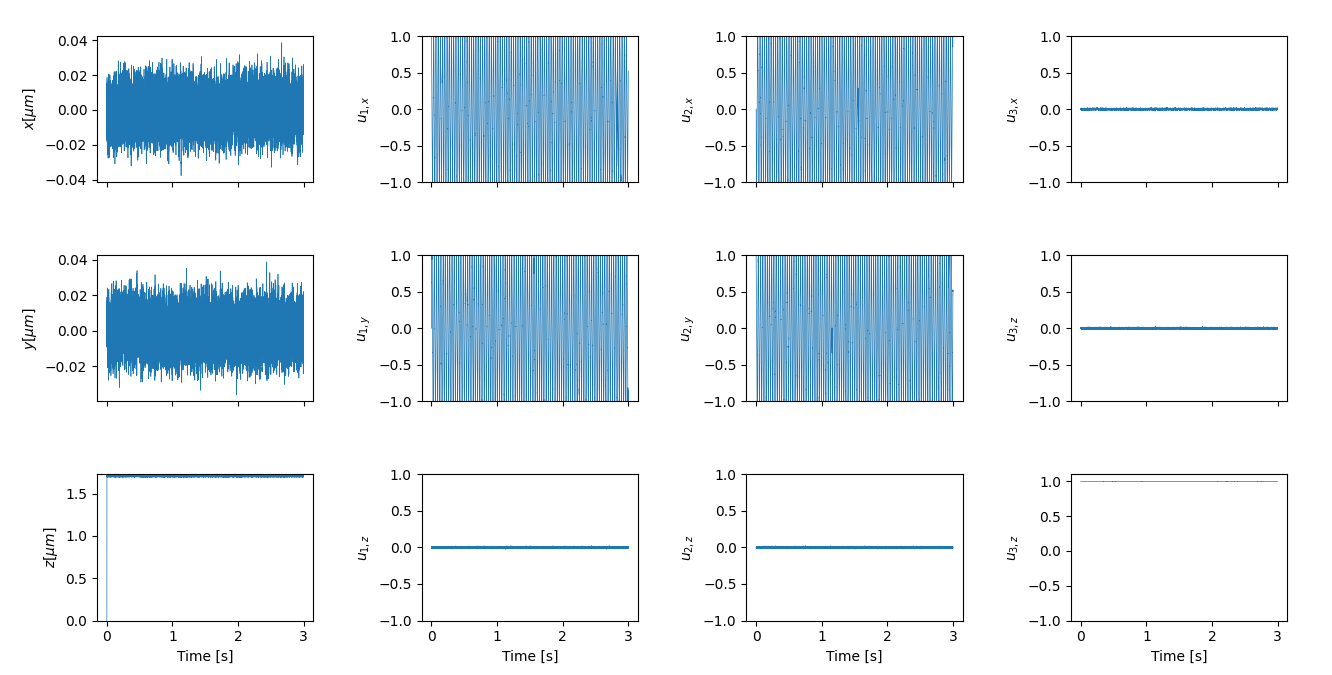
\includegraphics[width=\linewidth]{rotating_traj.png}
	\end{subfigure}
	$\downarrow$
	\begin{subfigure}{\linewidth}
		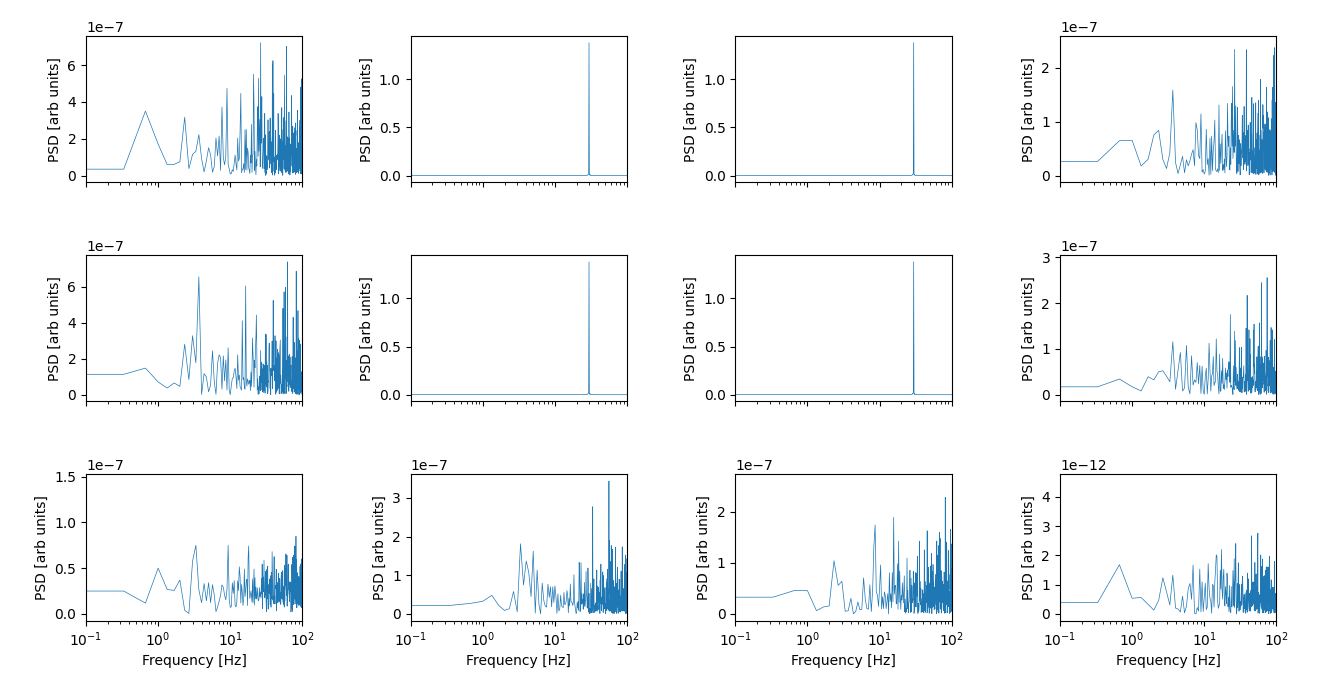
\includegraphics[width=\linewidth]{rotating_traj_fourier.png}
	\end{subfigure}
	\caption{Top: 3 second trajectory of a dimer trapped by a 
		circularly polarised Gaussian beam. The far left 
		column depicts the dimer's centre of mass position 
		with time; the remaining 3 columns show the 9 components 
		of the dimers' rotation matrix, with each column being
		associated with one of its three principal axis. Bottom: 
		The same trajectory but each time series has been 
		replaced with its Fourier transform. The only non-zero 
		elements are for the $U_{1,x}$, $U_{1,y}$, $U_{2,x}$, 
		and $U_{2,y}$ which show a single peak at the rotation frequency.} 
	\label{fig:fourier_transform}
\end{figure}

Each simulation was run for $1$ second ($\Delta t =10^{-5}\ 
s$) and at the end we looked at the orientational time series; 
the dimer's orientation is recorded as a quaternion which can 
be easily converted to a 3-dimensional rotation matrix. 
By considering only the transverse components ($U_{1,x}$, 
$U_{1,y}$, $U_{2,x}$, \& $U_{2,y}$) of the rotation 
matrix and taking the Fourier transformation of their 
time series reveals the rotational frequency. The 
laser power is set to $100\ mW$ to avoid large thermal 
fluctuations and so that the Fourier series of the 
transverse components approximates $\delta(\omega_
{rot}-f)$ - the Dirac delta function centred at the 
rotational frequency $\omega_{rot}$. This is 
demonstrated in fig.~\ref{fig:fourier_transform}

If the rotational frequency was not immediately obvious the 
simulation was repeated but over a longer simulation time. 
Four different size ratio of dimers were studied, both in 
their 'standard' and 'inverted' orientations. The results 
of this are displayed in Fig.~\ref{fig:rotation_vs_pol}:
\begin{figure}[h!]
	\centering
	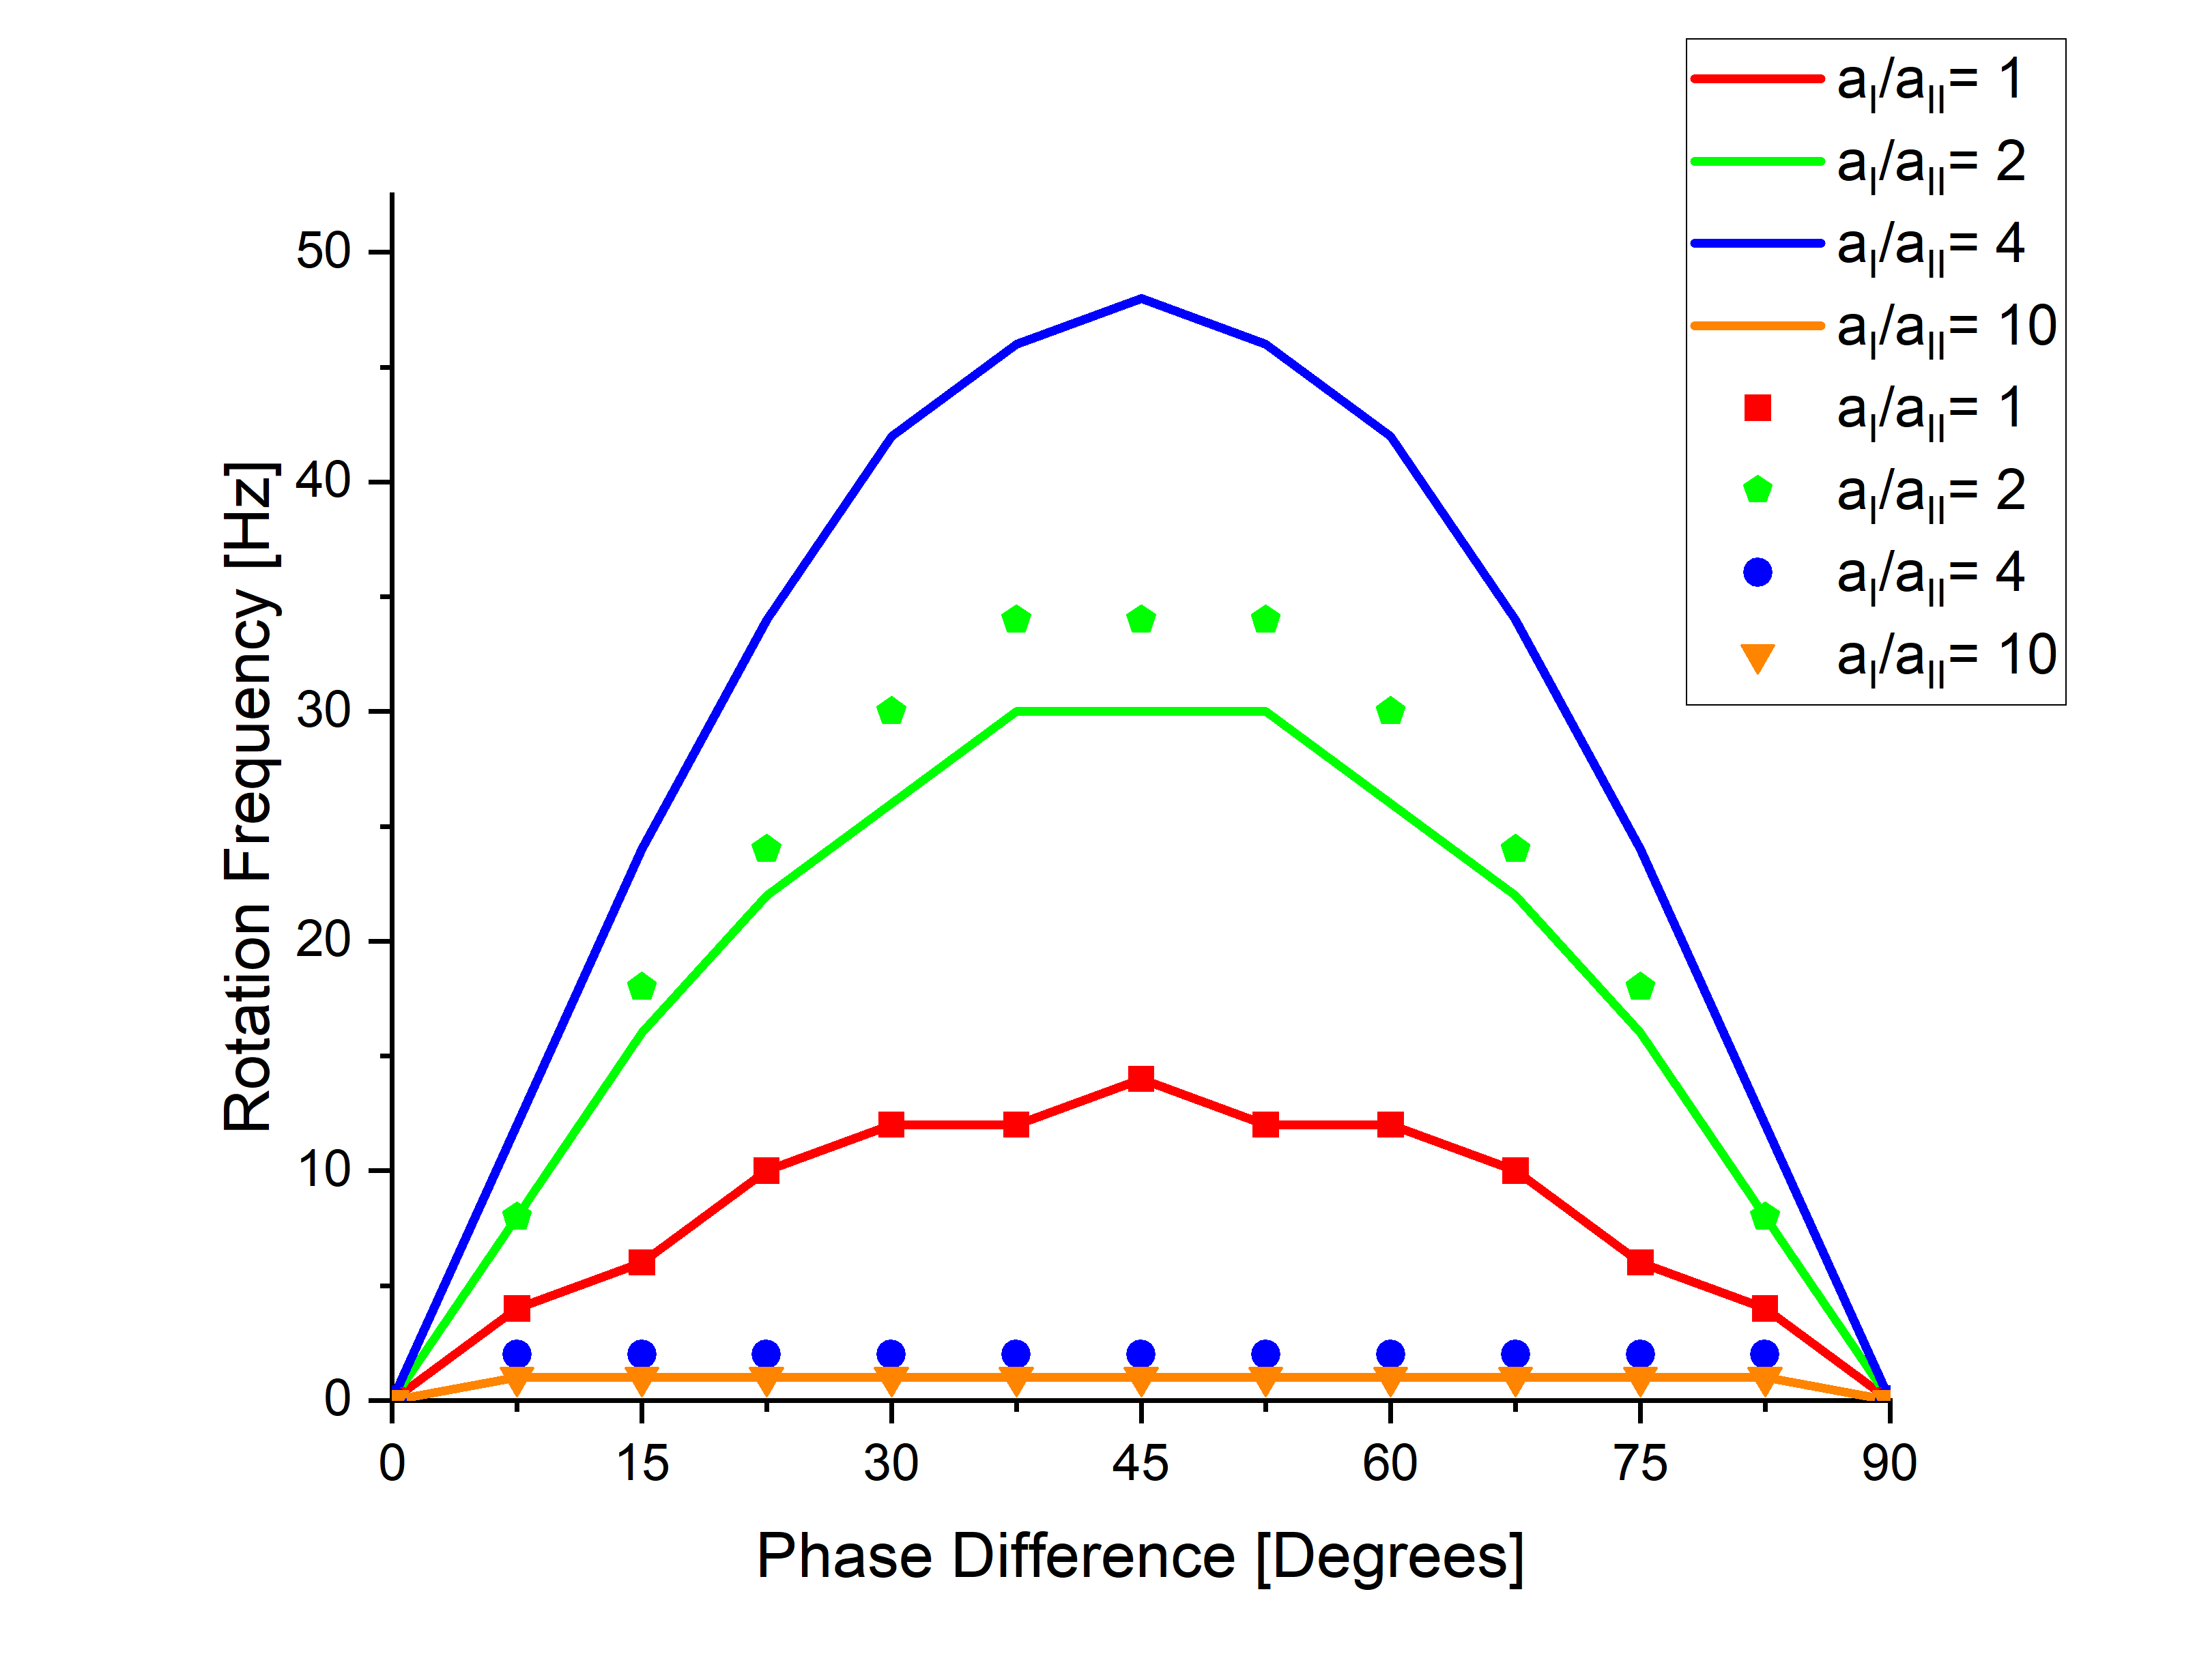
\includegraphics[width=0.9\linewidth]{rotation_rate_vs_pol.png}
	\caption{Rotation frequency vs electric field phase difference 
		for differently sized dimers. The solid lines represent 
		the rotation rate experienced while the dimer is in its 
		standard orientation, whereas the solid points are for 
		the case where the orientation is inverted. Laser power = 
		$100\ mW$.}
	\label{fig:rotation_vs_pol}
\end{figure}

This shows us that these optical rotations are polarisation 
dependent and not merely an example of the dimer scattering 
light asymmetrically. We also know that this cannot be a 
similar mechanism to that of experimental works \cite{Ahn2018, 
Reimann2018} as in our simulations the dimer's long axis
is parallel to the electric field. In this orientation 
the dimer's optical axis is aligned perpendicular to the
polarisation vector meaning that there should be no angular
momentum transferred along the optical axis. This is consistent 
with other experiments involving elongated particles. A dual
beam trap was used to study the dynamics of "disk like" particles. 
They found that these particles had one of two stable
orientations: Either orienting with the 'flat' side perpendicular
to the beam trap, with no rotation being observed \cite{Brzobohaty2015}. 
Or orientating with the 'flat' side parallel to the trap, in which 
case the long axis was aligned with the polarisation vector and 
thus rotational motion was detected \cite{Brzobohaty2015}.

\subsection{Brownian Vortex via Curl of Spin momentum}
In their work Vigilante refers to the spin-curl effects 
demonstrated by Grier \textit{et al} \cite{Ruffner2012}, 
in which the curl of the spin density leads to a second 
order optical force that orbits around the beams central 
axis \cite{Yevick2017}. While several papers have 
demonstrated this phenomena \cite{Zhao2007, Zhao2009, 
Wang2010} it was only properly formalised by \cite{Ruffner2012}. 
In which they showed that the seemingly random trajectory 
of a trapped sphere was biased by the polarisation state 
of the trapping beam. While not immediately evident from 
the trajectory the helicity of the trapping beam was revealed 
by computing the particle's probability flux using.
\begin{align}
	j(r) = \frac{1}{N-1} \sum_{j=1}^{N-1}
	\frac{r_{j+1}-r_j}{\tau}\delta_{sigma_j}\left(r-\frac{r_{j+1}+r_j}{2}\right)
	\label{eq:prob_flux}
\end{align}

where $\delta_{\sigma_j}$ is the kernel of an adaptive 
density estimator \cite{Silverman1986}. \eqref{eq:prob_flux} 
describes the direction a trapped sphere is most likely 
move in given our statistical knowledge of the 
trajectories probability density function. A finite 
estimation of the density function $p(r)$ is used in 
\cite{Ruffner2012}.
\begin{align}
	p(r) = \frac{1}{N}\sum_{j=1}^N \delta_{\sigma_j}(r-r_j)
	\label{eq:prob_density}
\end{align}

The probability flux reveals a biased motion in the trajectory 
of a single sphere (see Fig.~\ref{fig:Ruffner_Grier}). This 
biased motion results in a slight orbital motion about the 
central axis of the trapping beam, the orbital frequency is 
shown to be proportional to the polarisation state of the 
trapping beam. 
\begin{figure}[h!]
	\centering
	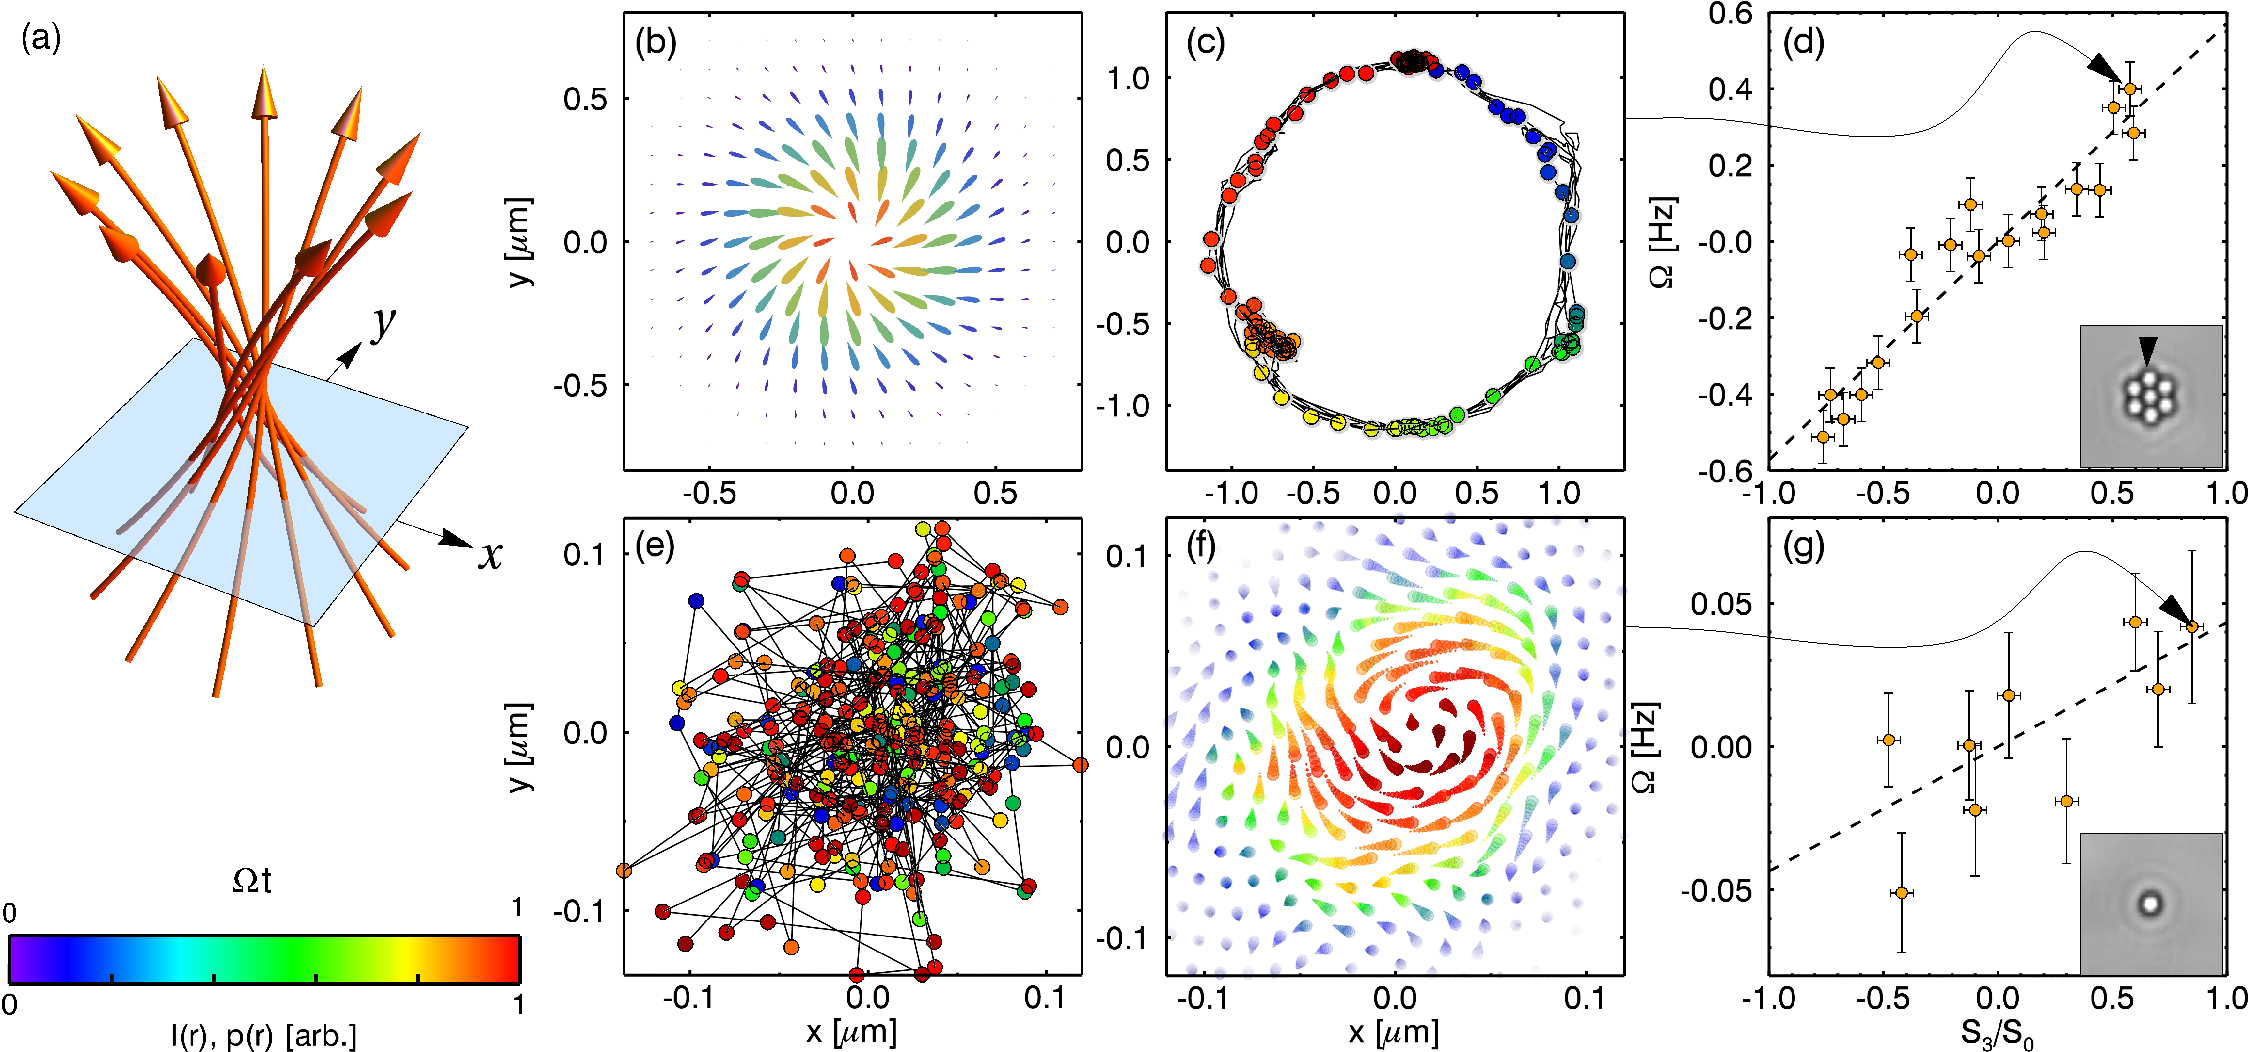
\includegraphics[width=\linewidth]{Ruffner_Grier_2012.pdf}
	\caption{Figure reused from \cite{Ruffner2012}. (a) shows how 
		the momentum density of a Gaussian beam is twisted while 
		using circularly polarised light. The top row (figures 
		(b)-(d)) shows a 7 sphere cluster trapped in a circularly 
		polarised beam. Due to the clusters asymmetric susceptibility 
		to polarization the cluster rotates in the $x-y$ plane. 
		Whereas the bottom row (figures (e) - (g)) show the similar 
		results for a single sphere. In this instance the sphere 
		does not rotate but instead orbits the beam axis. In both 
		instances the motion is proportional to the degree of 
		polarisation (see figures (d) and (g)) but for the single 
		sphere this motion is only revealed when using 
		\eqref{eq:prob_flux} \& \eqref{eq:prob_density}. Reused 
		with permission from author}
	\label{fig:Ruffner_Grier}
\end{figure}

While the results from \cite{Ruffner2012} suggest that the 
optical rotation seen in asymmetric dimers can be attributed to 
the same spin-curl forces there are several questions that 
cannot be explained purely by the spin-curl force. 

\subsection{Optical torque differences}
In their paper Grier \textit{et al} show that a 7 sphere cluster
will rotate when trapped in circularly polarised light but a 
homogenous sphere will have a slight curl to its trajectory. 
They attribute this to the curl of the spin angular momentum
generating a "Brownian vortex". But what is more interesting, 
and something that appears unaddressed, is how the effects of 
this vortex change based on the overall shape of the target
particle.

You would not expect that the addition of a single additional 
sphere should drastically adjust the torque especially if said 
sphere is relatively small. However when we measured the optical 
torque of a single sphere and a dimer - $a_{I}/a_{II}=10$ - we 
found the exact opposite. In both cases we used the same trapping 
beam as used for fig.~\ref{fig:rotation_vs_pol} but with a 
circularly polarised beam. Both the sphere and dimer were rotated 
in the $x-z$ plane and the all three components of the optical 
torque were recorded.
\begin{figure}[h!]
	\centering	
	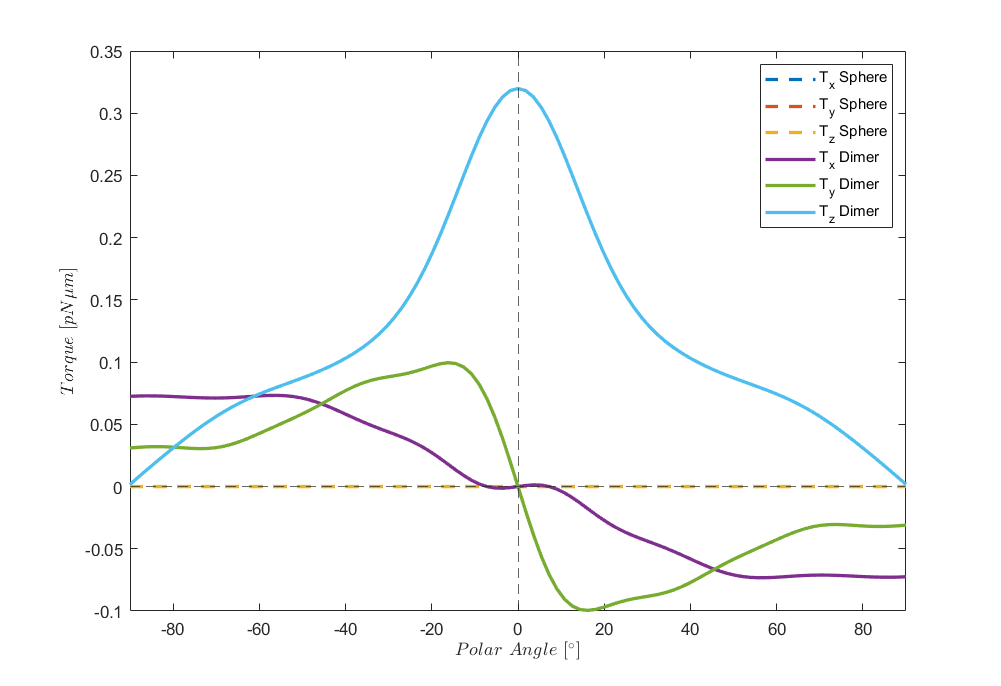
\includegraphics[width=\linewidth]{sphere_dimer_torque.png}
	\caption{Optical toque experienced by a dimer ($a_{I}/a_
	{II}=10$) and a single isotropic sphere. Both were rotated 
	in the $x-z$ plane and the angle between $U_z$ and the beam 
	axis gives the polar angle.The solid lines denote the torque 
	experienced by the dimer whereas the dashed lines represent 
	the torque experienced by the sphere.}
	\label{fig:sphere_dimer_torque}
\end{figure}
 
The torques about the $x$ and $y$ axis can be somewhat understood 
as the second sphere is being drawn back towards the centre of the 
trap by the gradient forces. The same cannot be said for the $z$-
component of the optical torque, which is non-zero even at a 
$80^\circ$ angle. This cannot be simply explained via spin-curl 
effects, as the 'Brownian vortex' should instead be driving the
dimer around the beam axis - similar to how the 7 sphere cluster 
behaved. What is clear that the mere combination of two spheres
results in a unique behaviour that has not been previously 
investigated. 

\subsection{Rotational frequency as a function of size ratio and 
	orientation}
\label{sec:rot_size}	
One factor t Intuitively, you would expect that a 
larger particle would experience a greater torque and therefore 
rotate faster. By repeating the same kinds of simulation as used 
in \ref{fig:rotation_vs_pol} but for a circularly polarised beam 
$\phi=90\circ$ it was found that not only is the rotation rate 
dependent on the size of the dimer, but also on its orientation 
and therefore their axial position.
\begin{figure}[h!]
  \centering
  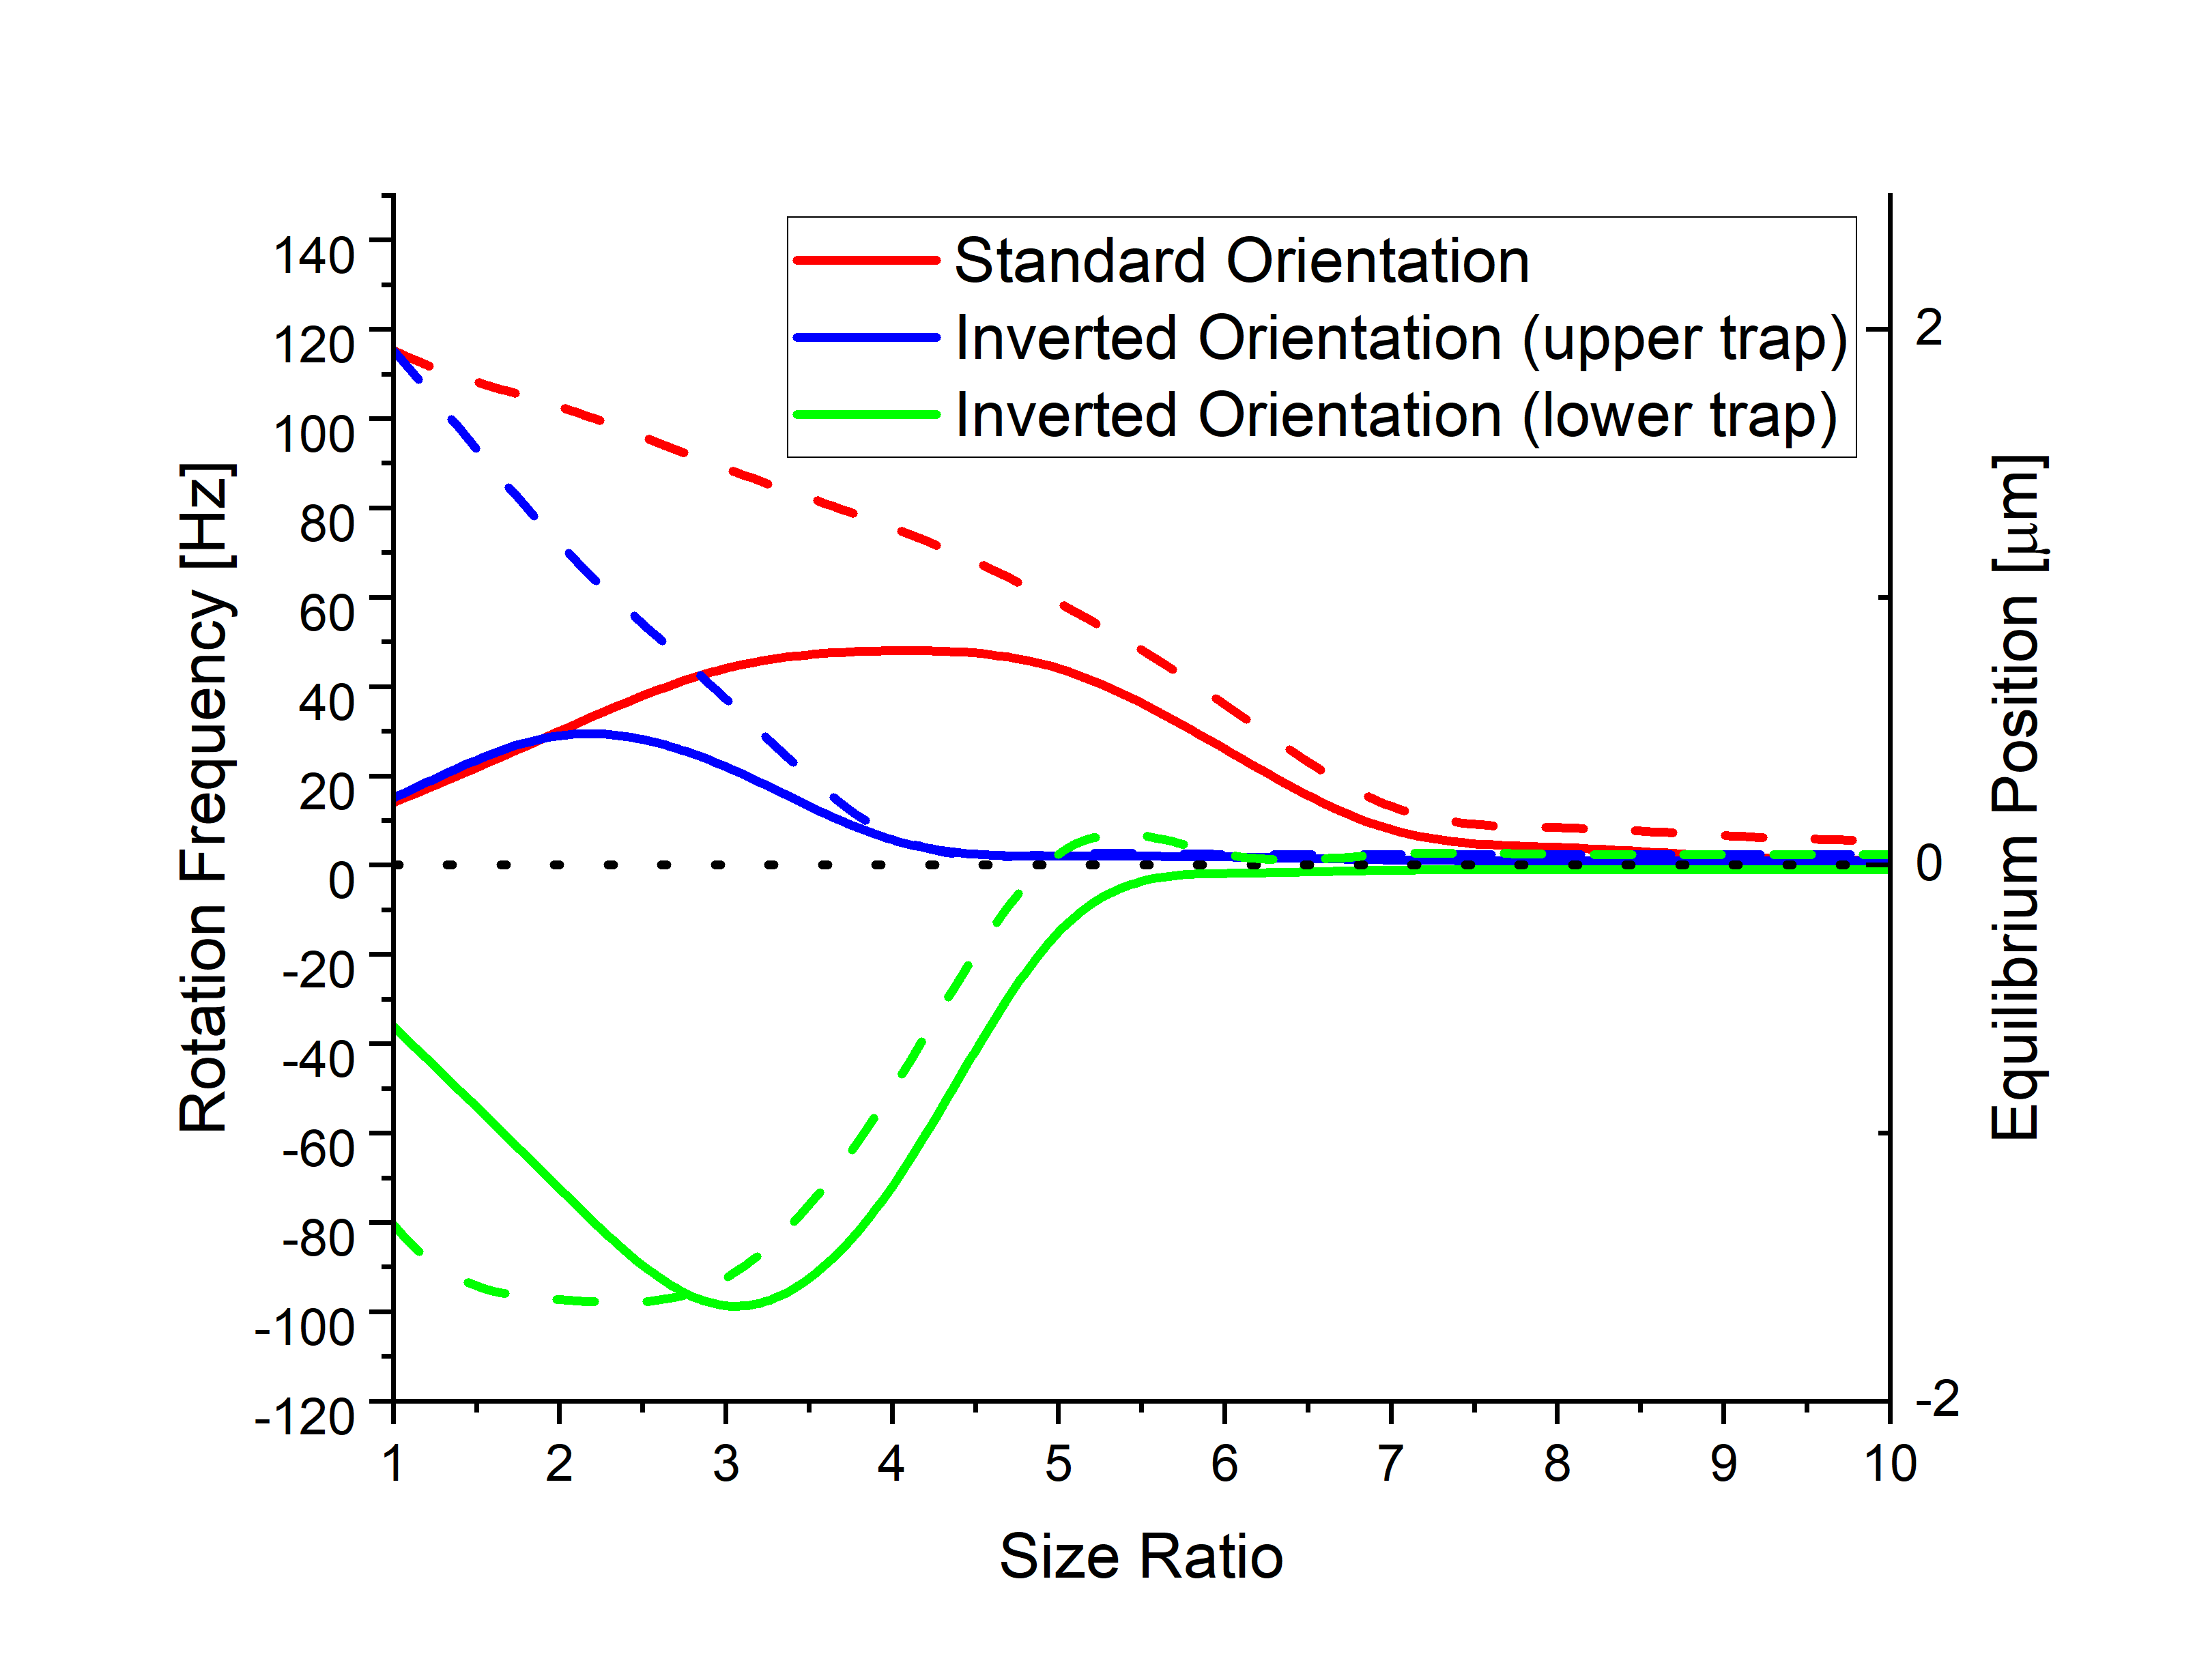
\includegraphics[width=\linewidth]{rotation_rate_vs_size.png}
  \caption{Rotation rate plotted against dimer size ratio while 
  	trapped in a circularly polarised beam; a positive rotation 
  	rate indicates clockwise rotation, whereas a negative 
  	rotation rate indicates counter-clockwise rotation. The red 
  	line is for the case of a dimer in its 'standard' orientation. 
  	The blue line is for the case when the dimer is in its 
  	'inverted' orientation while trapped above the focus of the 
  	beam. And lastly the green line is for the case when the 
  	dimer is in its 'inverted' orientation, but when it is trapped 
  	below the focus of the beam.}
\end{figure}

It is difficult to see from the graph, but the rotation rate never
truly goes down to zero, reaching a minimum of $2\,{\rm Hz}$, which 
would imply that a second sphere of radius $200\,{\rm nm}$ is enough 
to induce rotational motion. It is not clear if the optical torque 
calculated for the larger size ratios is accurate as you would not 
expect the rotation rate to plateau like this. From fig.~
\ref{fig:sphere_dimer_torque} it seems clear that the torque is not
merely an error of the numerical calculations as it would not have 
such a strong angular and positional dependence. Most likely with 
longer simulation times would reveal the real relationship behind
the rotation rate and the size ratio. 

What is also interesting is that the rotation rate is not correlated 
directly with either the particle size or the equilibrium position. 
This is in stark contrast to previous reports of dimer optical 
rotation; Ahn \textit{et al.} reported that the rotational frequency 
is maximised when the dimer is symmetric \cite{Ahn2018}. Their work 
was conducted experimentally in a vacuum so the only limiting factor 
to the optical rotational motion is the structural stability of the 
particle itself. 

\subsection{Gyroscopic Precession using asymmetric dimers}
As mentioned in section~\ref{sec:off-axis} for specificity sized 
dimers there is the potential for non-vertical trapping orientations 
in which the dimer is still stably trapped. When a circularly 
polarised beam is used the dimer exhibits gyroscopic precession. 
As shown in fig.~\ref{fig:gyro} the dimer's trajectory exhibits 
periodic rotation, both around its long axis and about the beam 
axis.
\begin{figure}[h]
	\centering
	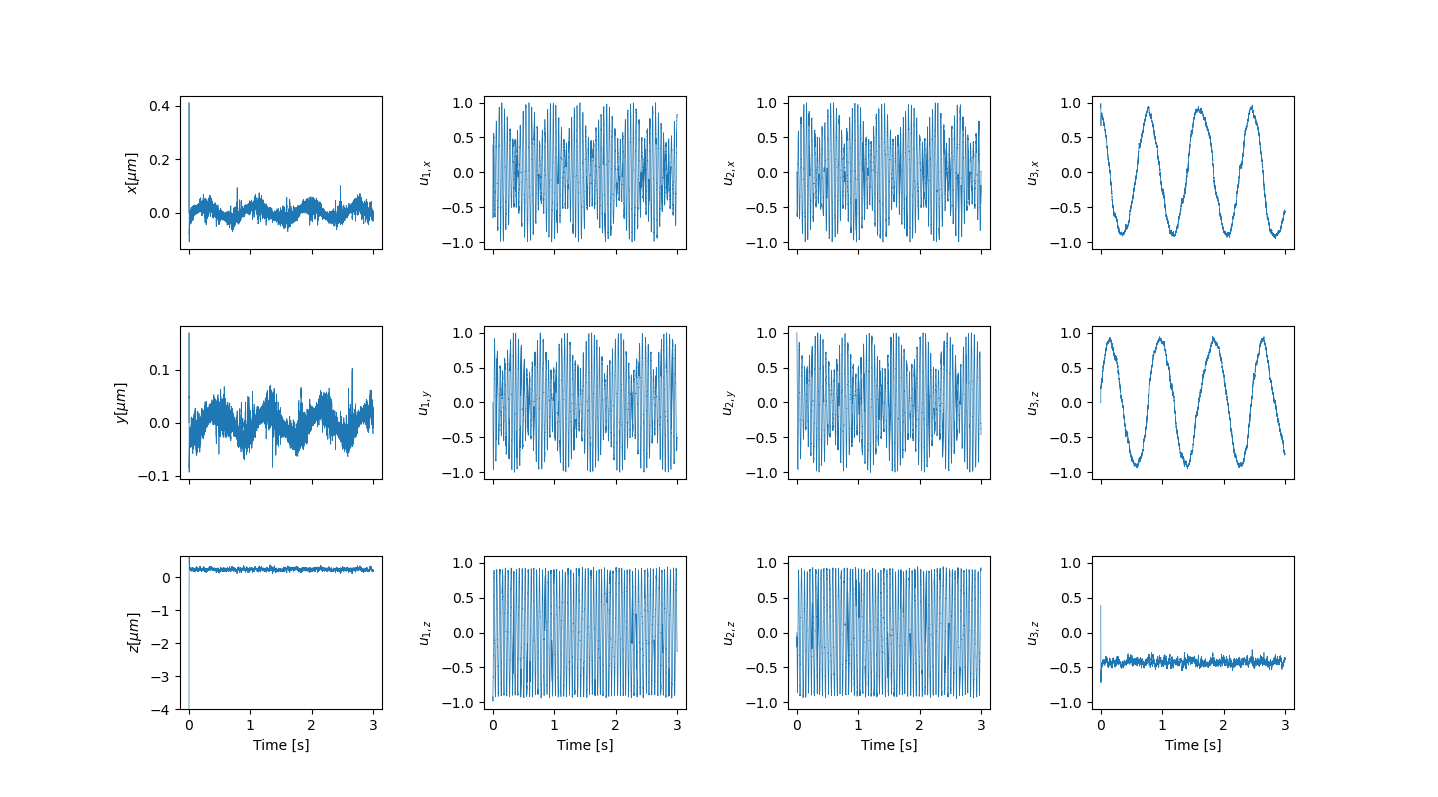
\includegraphics[width=\linewidth]{gyroscopic_precession.png}
	\caption{3 second trajectory of a dimer ($a_{I}/a_{II}=2$) trapped 
		in an off axis orientation with a circularly polarised beam 
		($P= 100\ mW$). The far left column depicts the dimer's centre 
		of mass position with time; the remaining 3 columns show the 9
		components of the dimers' rotation matrix, with each column being
		associated with one of its three principal axis.}
	\label{fig:gyro}
\end{figure}

Applying a Fourier analysis to the above trajectory reveals 
the 3 fundamental frequencies typically associated with 
gyroscopic precession. Fig.~\ref{fig:gyro_diagram} gives 
a representative idea of the motion seen in fig.~\ref{fig:gyro}.
Firstly there is precession, is denoted by $\psi$, this
causes the dimer to rotate in the $XY$ plane while maintaining
a constant polar angle. The precession can be due to the dimer 
having inhomogeneous polarisation susceptibility. Since its 
long axis is more susceptible to being polarised the dimer will
try to align its long axis with the polarisation vector 
\cite{Bruce2020}. Second there is nutation, denoted by $\theta$, 
which is due to the dimer's Brownian motion being influenced by 
the 'Brownian vortex', as predicted by \cite{Ruffner2012}. And 
lastly there is rotation, denoted by $\omega$, where the dimer
spins around its long axis as it did in \ref{sec:rot_pol} \&
\ref{sec:rot_size}. If the rotation was due to the curl of the 
spin angular momentum then you would only expect to see 
precession and nutation, the addition of rotational motion 
suggests that having multiple particles in close proximity 
results in a transfer of angular momentum along the long 
axis.
 
What is interesting is that while we see the precession and 
nutation also contribute to the rotation frequency. As can be 
seen in both fig.~\ref{fig:gyro} and fig.~\ref{fig:gyro_diagram}
the rotation matrix components $U_{x,x}$, $U_{x,y}$, $U_{y,x}$
and $U_{y,y}$
\begin{figure}[h!]
	\hspace{-2.3cm}
	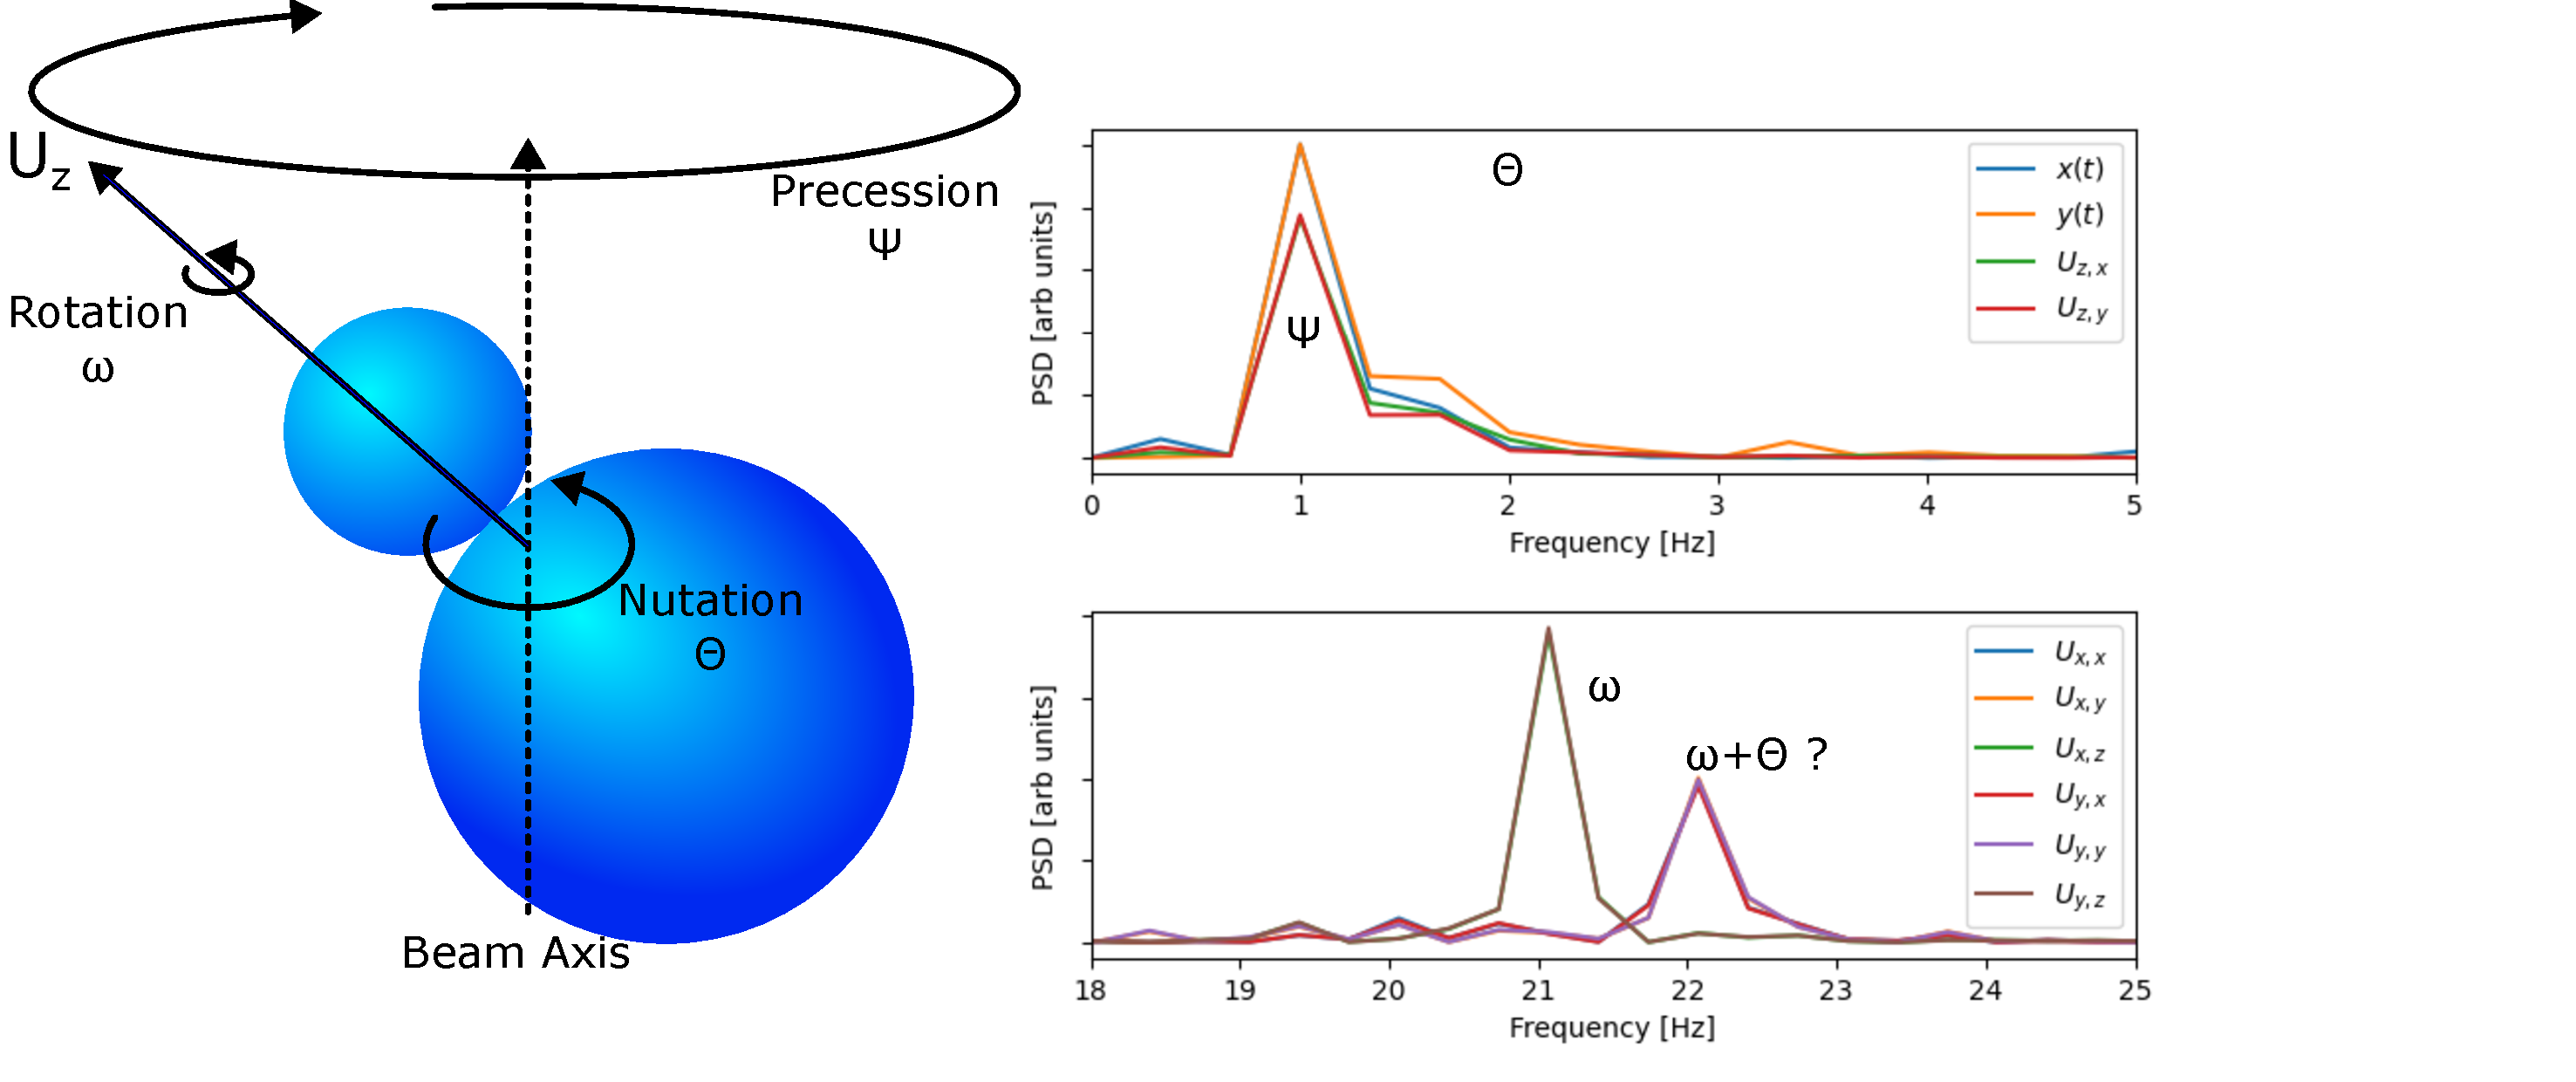
\includegraphics[width=1.2\linewidth]{gyroscopic_diagram.pdf}
	\caption{Representative diagram of the gyroscopic precession 
	from fig.~\ref{fig:gyro}. The dimer has three principal angular
	frequencies: The rotation ($\omega$) occurs around the 
	the dimer's long axis. Precession ($\psi$) is seen where the dimer 
	rotates around the beam axis. Nutation ($\theta$) is due to the dimer's 
	centre of diffusion orbiting the beam axis. Shown on the right
	is the power spectra from fig.~\ref{fig:gyro} with the associated 
	frequencies labelled. The power spectrum have been zoomed in on
	the relevant frequencies to highlight the precise values.}
	\label{fig:gyro_diagram}
\end{figure}

This gyroscopic motion has been demonstrated previously in 
nanoparticles \cite{Zhu2021, Rashid2018, Hoang2016, Kuhn2016} 
but has not been observed for micron scale aggregates. What
is interesting that the precession is seen around the particle's
optical axis (in the case of a dimer this would be its long 
axis). Fig.~\ref{fig:gyro} instead shows the precession 
occurring perpendicular to the optical axis. In the former 
case the precession was explained as simply occurring due 
to the reaction torque from the surrounding fluid \cite{Zhu2021}.
In their analysis of ellipsoidal particles, Zhu \textit{et al.}
found that when the particle rotated around their minimal inertial 
axis (similar to the observed behaviour in dimers), the particle 
would quickly 'stabilise' by aligning its' optical axis with the 
beam axis. This highlights that a spherical dimer is capable of 
rotating about its minimal inertial axis while remaining stably
trapped. This has potential implications beyond simply 
understanding particle dynamics. 

Further analysis of the mechanism behind the precession of off-axis 
dimers may provide insights into controlling Brownian motion. An 
experimental work trying to 'cool' nano-dimers by controlling the 
motion in all 6 degrees of freedom found that even while the 
rotation about the short axis' could be controlled the free rotation 
around the dimers' long axis resulted in an unpredictable torsional 
vibration \cite{Bang2020}. Understanding how rotational motion 
arises in the Mie-regime could allow researchers to build a robust 
theoretical framework to construct beam structures that eliminate any 
unwanted rotational motion from a target particle. Conversely, the 
same framework could allow for precise measurements of the optical 
torque applied to a target particle, allowing for characterisation 
of complex shaped particles' interactions with an optical trap. 

%%%%%%%%%%%%%%%%%%%%%%%%%%%%%%%%%%%%%%%%%%%%%%%%%%%%%%%%%%%%%%%%%%%%%%%%%%
%%%%%%%%%%%%%%%%%%%%%%%%%%%%%%%%%%%%%%%%%%%%%%%%%%%%%%%%%%%%%%%%%%%%%%%%%%

\section{Conclusions}
Considering the simplicity of a scatterer such as a dimer, 
one would assume that the dynamics of such an object would 
be relatively easy to predict. Simulations of dimers in 
the Mie regime show that not only do they have multiple 
positions and orientations in which they can be trapped but 
also that their interaction with circularly polarised light 
is heavily dependent on the axial position and trapping 
orientation. 

Dimer's have the potential to be used as tunable micro-rotors, 
being simple to synthesise and can be made out of any material 
of choice. The rotation demonstrated by dimer's is not accurately
described in previous literature which raises questions on the
interactions between circularly polarised light and spherical 
aggregates. Until now, our understanding of angular momentum 
transfer has been either focused on single particles (where 
momentum transfer is easily described by Lorenz-Mie theory) or 
for large aggregates of particles, where the angular momentum 
transfer between individual particles is not considered. This 
could provide a greater understanding of angular momentum and 
help in the development of better torque sensing or torque 
preventing methods.

